\chapter{Data Quality Monitoring using Deep Learning techniques}
\label{chap:Results}

This chapter will run through the actual process of implementing the algorithm to perform data quality monitoring tasks.
We begin with a brief introduction to DQM, then discuss reference and data samples, technicalities about NN parameters
and, finally, the results of this work.

\section{Data quality monitoring}\label{sec:DQM}

Where there is data, there is the risk of bad data, and bad data is expensive. It could be expensive in terms of time,
but also terms of money. To ensure that the data being collected is of reasonable quality, we need to monitor data and
get notified in time to correct whatever is damaging our data quality, or, even better, have the whole monitoring
process automated. The latter is what we aim to achieve, but it is a steep path. 

Ideally, we would look for a fully automated, online data quality monitor. In other words, we would like to have an
algorithm that independently recognizes whether the collected data is acceptable or not while the detector is collecting
data. Moreover, the algorithm would raise a warning or an error whenever data is of poor quality, depending on how
dangerous the quality loss may be. Eventually, we would have it take action and even shut down the detector if
necessary. 

We have been focusing our attention on the very first part of the last two sentences during this thesis work. Namely, we
wanted to have an algorithm that can discriminate between good quality and bad quality data. Unfortunately, tests have
been performed offline, meaning that data had already been collected, and no automation aside from the actual
recognition has been implemented.  

\section{Monitoring the time box}

As briefly anticipated at the end of \autoref{s:DriftTime}, the data distribution chosen to be our test case is the time
box, the distribution of electrons' drift times. This choice was not made by chance: time box distribution features,
such as the overall shape, tails and edges, are correlated to the correct working of the detector (i.e., if the detector
has some failures, those can be spotted in a time box showing statistically significant departures from the expected
distribution).

\subsection{Experimental datasets}\label{sec:exp_timebox}

In the time frame in which we have worked on this thesis, the detector has collected almost $100\,\text{Gb}$ of data
acquired in multiple runs. These runs are different as they have been used to perform other tests on the experimental
setup settings. However, the specifics of the runs were not known by us, so we had a flat prior to the distributions,
and it was impossible to introduce any bias towards them. It seemed a good plan to us, as the whole work has been
carried out in a model-independent framework.
%  On the other hand, this made it impossible to study quantitatively how an
% incorrect choice of experimental settings, and its corresponding malfunctioning of the detector, leads to a discrepant
% distribution of the drift times. 

Hence, to choose a few distributions on which to do our monitoring tests, we could not simply pick a detector's run with
known working settings as our reference dataset and select others that did not share such settings. Thus, we first
selected the runs that collected noticeably larger datasets (e.g., usually $\sim 20$ hours runs or shorter ones
collected at a higher rate). Then, we have analyzed the time box of each of those high statistics runs: our physics
background and the standard working conditions suggested that the drift times distribution should be almost uniform,
ranging from $0$ to $400\,\si{\nano\second}$ (as previously explained in \autoref{s:DriftTime}). We realized that all
the time boxes analyze could fit in three categories: \textit{good}, \textit{discrepant} and \textit{bad} runs. 

Good runs are those that agree with our expectations, both in shape and width. Discrepant runs show some departures from
the expected distribution, either in shape or width. Bad runs do not follow our predictions, both in shape and width. To
clarify, in \autoref{fig:dt_cat} are shown four examples of time boxes. Those four distributions are the ones being
tested.

\begin{figure}[h]
    \begin{subfigure}[b]{0.5\textwidth}
        \centering 
        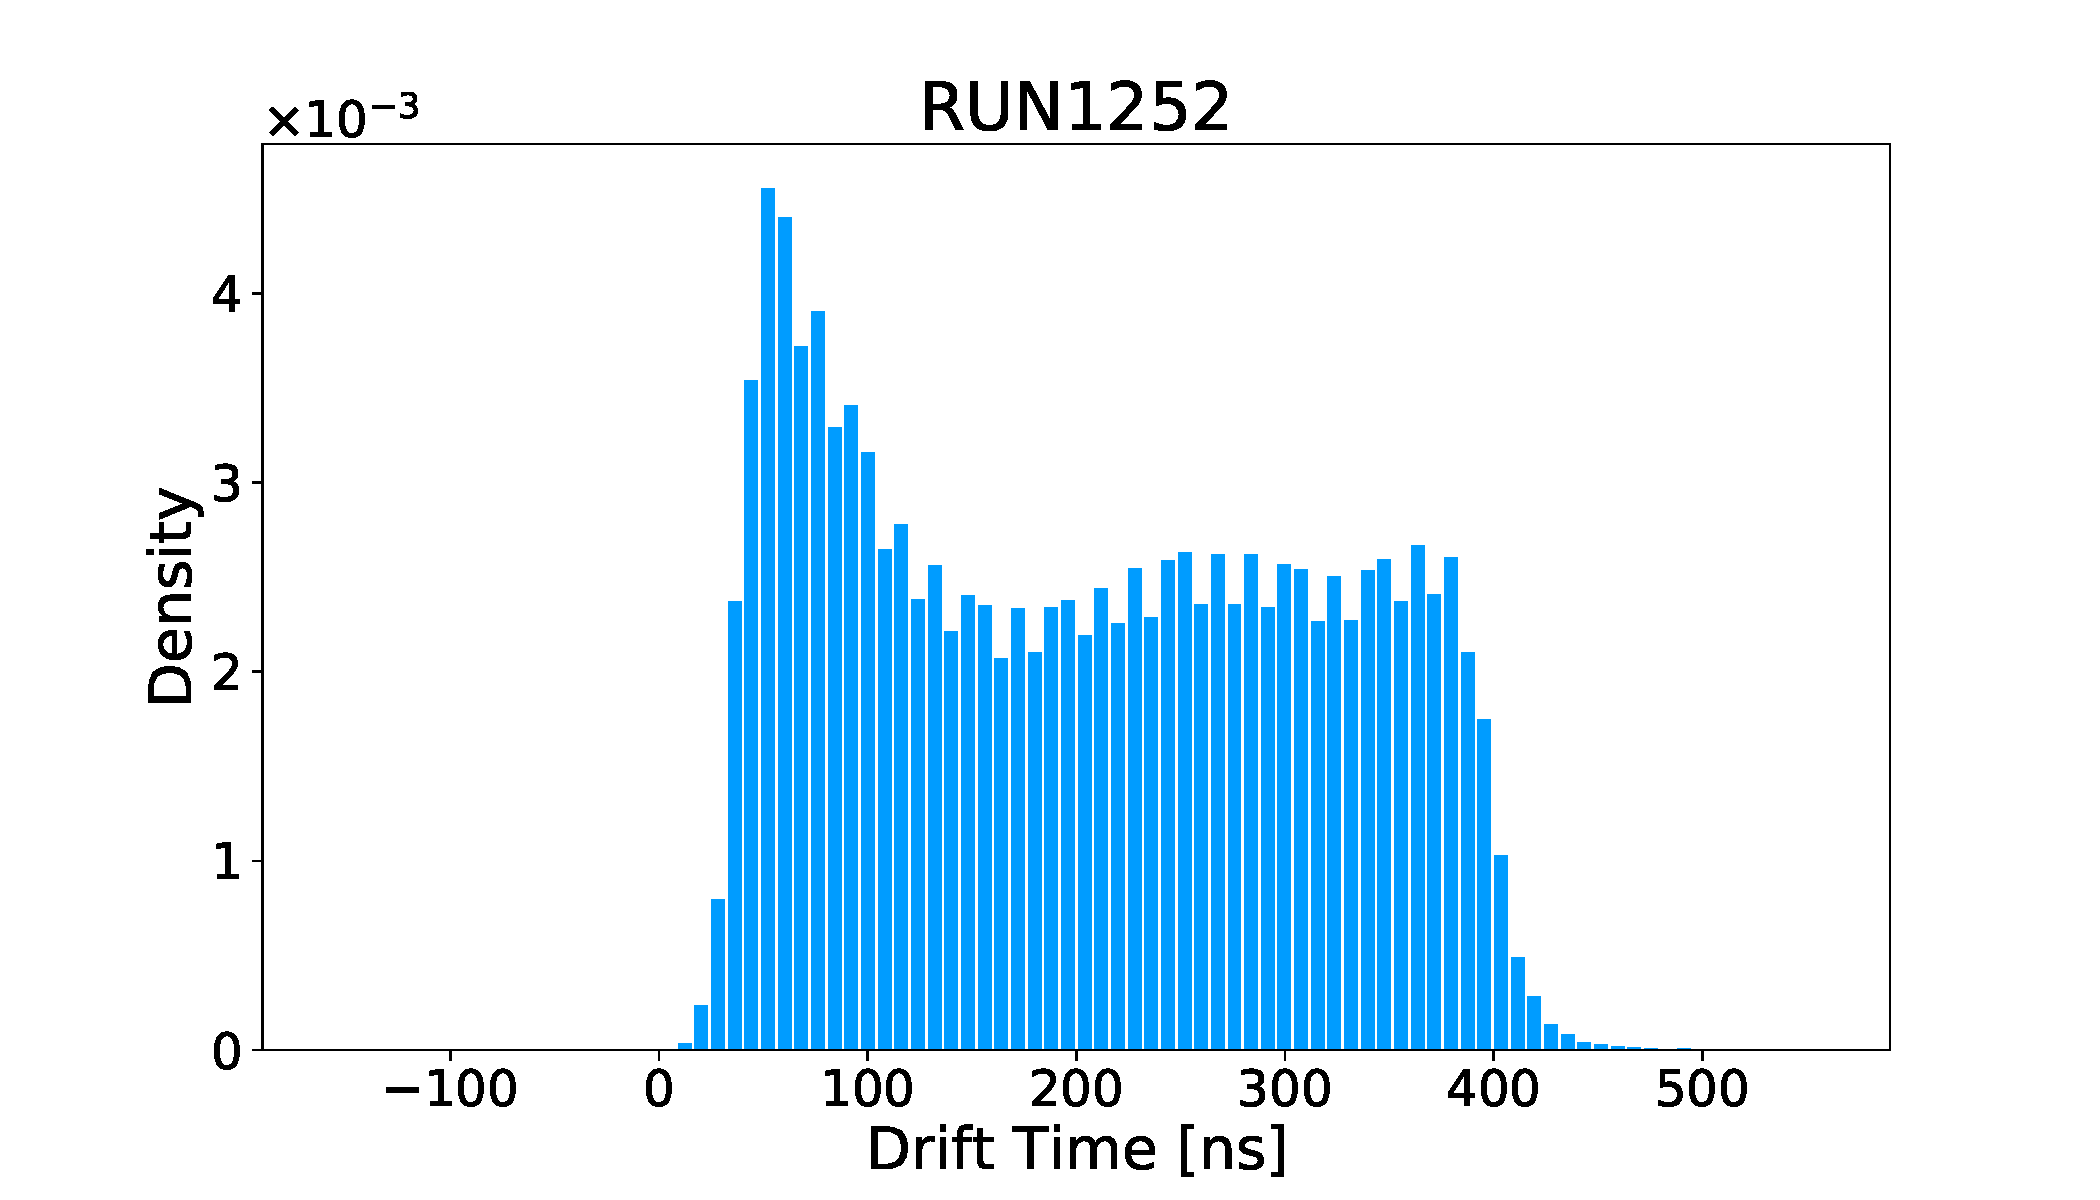
\includegraphics[width=1.0\textwidth]{./Images/experiment/RUN1252.pdf}
        \caption{Good distribution}
        \label{fig:dt_cat:a}
    \end{subfigure}%
    \hfill
    \begin{subfigure}[b]{0.5\textwidth}
        \centering 
        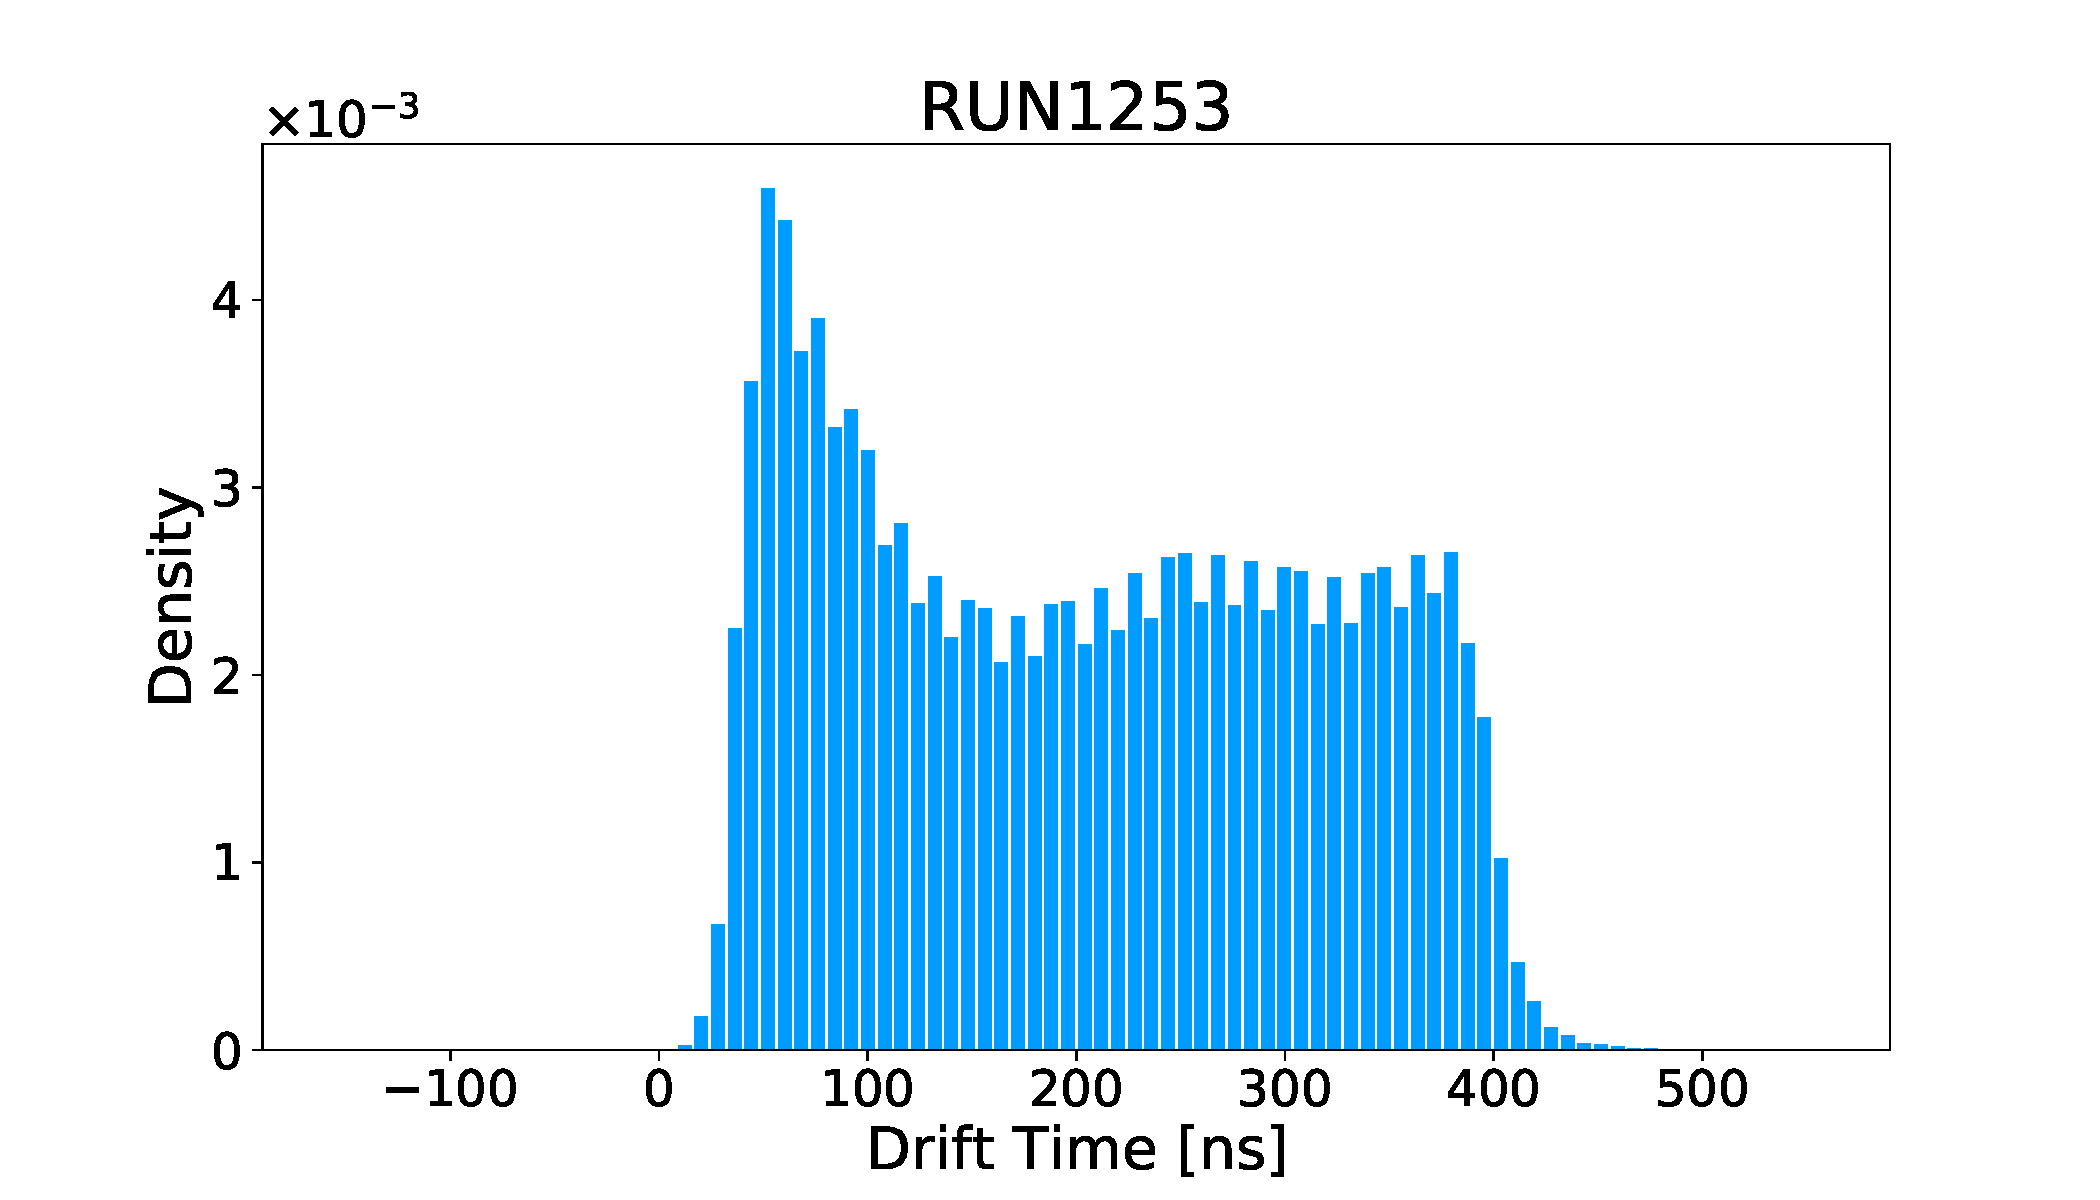
\includegraphics[width=1.0\textwidth]{./Images/experiment/RUN1253.pdf}
        \caption{Good distribution}
        \label{fig:dt_cat:b}
    \end{subfigure}%
    \\
    \begin{subfigure}[b]{0.5\textwidth}
        \centering 
        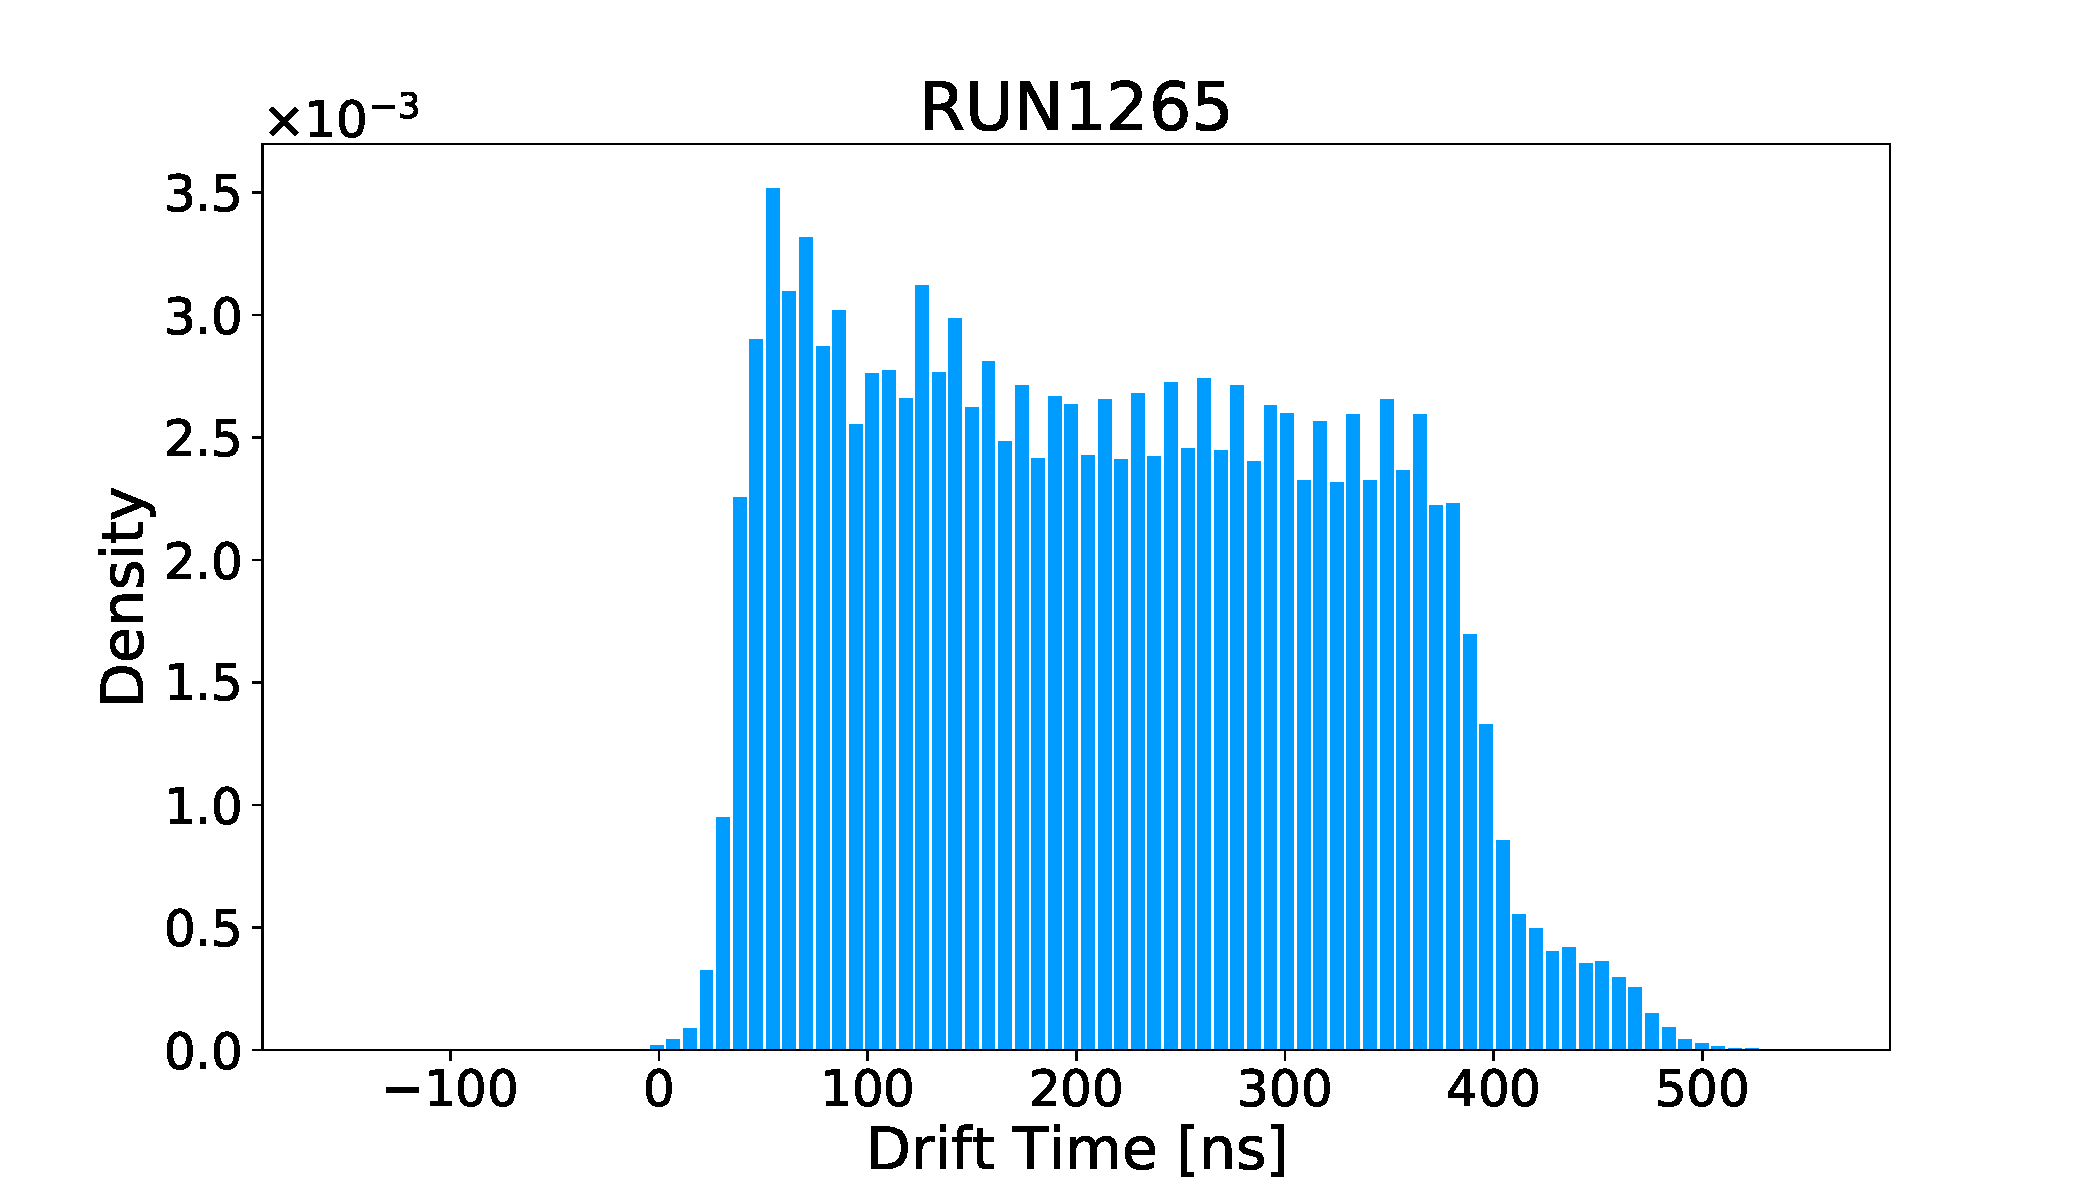
\includegraphics[width=1.0\textwidth]{./Images/experiment/RUN1265.pdf}
        \caption{Discrepant distribution}
        \label{fig:dt_cat:c}
    \end{subfigure}%
    \begin{subfigure}[b]{0.5\textwidth}
        \centering 
        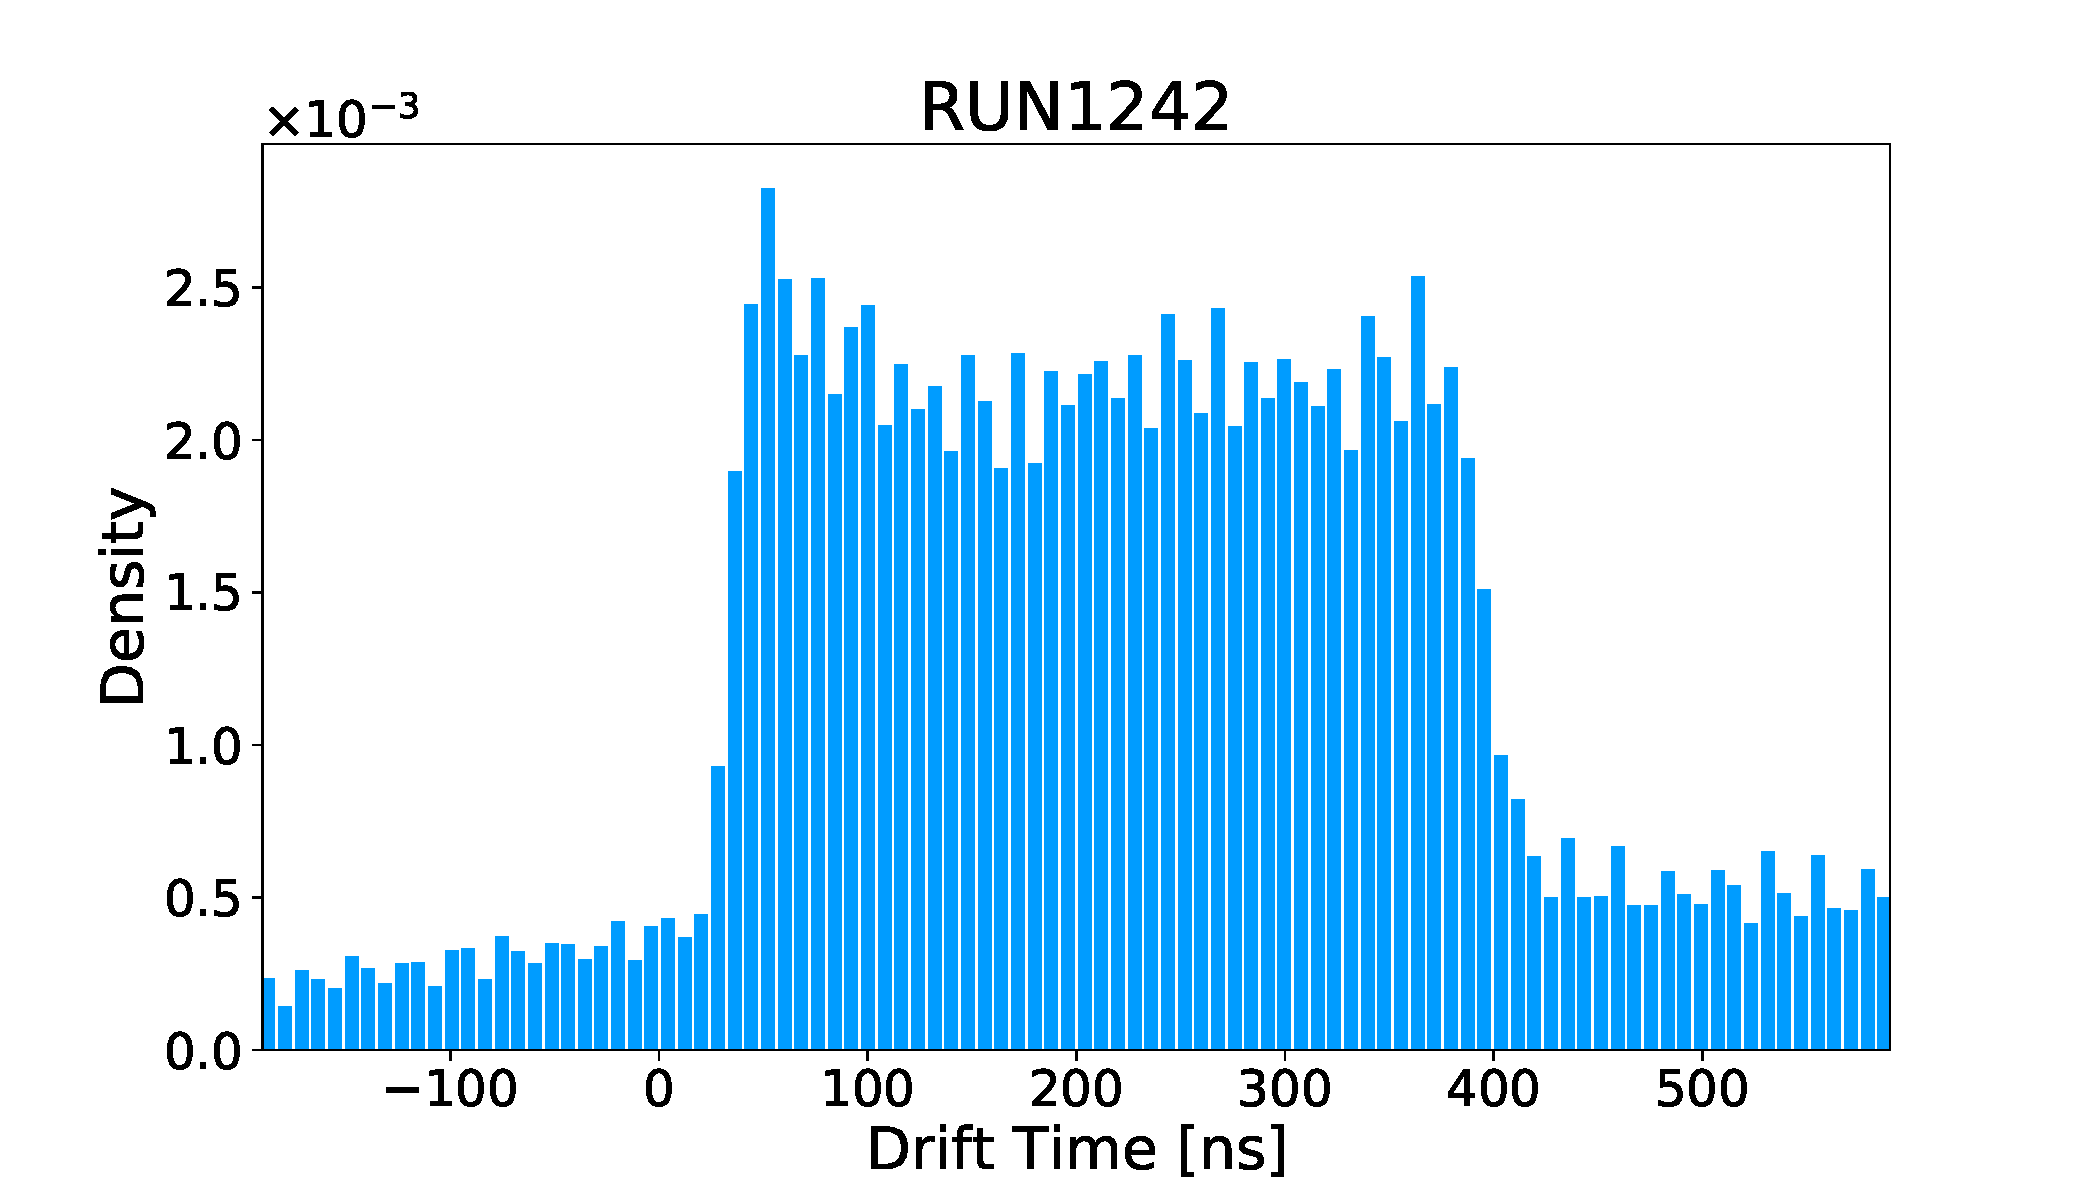
\includegraphics[width=1.0\textwidth]{./Images/experiment/RUN1242.pdf}
        \caption{Bad distribution}
        \label{fig:dt_cat:d}
    \end{subfigure}%
    \caption{Time boxes tested with our deep learning algorithm}
    \label{fig:dt_cat}
\end{figure}

Briefly, \autoref{fig:dt_cat:a} and \autoref{fig:dt_cat:b} are both \textit{good} runs. Note that they share a peak
placed on the left edge of the distribution, caused by the detector's geometry, which is also expected. The fact that
RUN1252 and RUN1253 look the same when plotted using a 100-bins histogram tells us that statistical fluctuations are
almost imperceptible to sight with that amount of data. On the other hand, \autoref{fig:dt_cat:c} falls into the
\textit{discrepant} category: though the overall shape is almost acceptable, the right-hand tail is noticeably out of
range. Finally, it is more than evident that \autoref{fig:dt_cat:d} does not agree with our expectations at all: it
seems that the detector collected a relevant background noise component that ruined the width of the distribution.


\section{Implementing the deep learning algorithm}

Referring to \autoref{fig:summary} in \autoref{sec:overview}, the algorithm takes as input two distributions: the
reference sample $\R$ and the data sample $\D$. Thus, in our scenario, we first needed to identify a reference
distribution: it made sense to choose as $\R$ data coming from a \textit{good} run: this way, the neural network would
compare any given $\D$ with our idea of what a time box should be. We have selected RUN1252 (\autoref{fig:dt_cat:a}) as
our reference run. 

Then, before testing the algorithm's performance on the remaining three drift time distributions, we had to build the
deep learning model: the architecture of the network, its activation functions, the optimizer. After that, NN's
hyperparameters were to be tuned: we need to ensure some degree of compatibility between the distribution of the test
statistic $t$ under the null hypothesis and the $\chi^{2}_{\nu}$ distribution, where $\nu$ stands for the degrees of
freedom of the network. Thus, the standard procedure for optimizing hyperparameters involves feeding the algorithm with
the reference $\R$ and a sub-sample $\D_\R$ for many different $\D_\R$s. Then, testing for the compatibility between
$p(t\,|\,\mathbfcal{R})$ and $\chi^{2}_{\nu}$, and repeating the procedure with different values for the hyperparameters
until satisfactory compatibility is reached. 

\subsection{Technical implementation of the model}

A sufficient amount of $\D_\R$ distributions sampled from the reference dataset are necessary to tune the network
hyperparameters successfully. Moreover, a changing yet significant amount of training epochs are needed to reach good
compatibility with the expected $\chi^2_{\nu}$ distribution. Thus, running the algorithm turns out to be computationally
heavy: tasks parallelization or distribution is mandatory to achieve the desired results in a reasonable amount of time.
Then, a cluster of machines, located in Legnaro and Padova, was used, and jobs were submitted via Condor. The t2-ui-12
machine was accessed via ssh tunnel through the INFN gate to submit the jobs to the batch system.

The algorithm has been implemented in Python using the Keras module. The optimizer used to minimize the loss function is
ADAM, as implemented in Keras with the TensorFlow backend, with an initial learning rate set to $10^{-3}$ and parameters
$\beta_1=0.9$, $\beta_2=0.99$, $\epsilon=10^{-7}$. The batch size has been kept fixed to cover the whole training sample
throughout the work. 

\begin{figure}[h]
    \centering
    % Fully Connected Neural Network

\def\layersep{2.5cm}
\resizebox{!}{0.35\paperheight}{%
\begin{tikzpicture}[shorten >=1pt,->,draw=black!50, node distance=\layersep, scale=0.5]
    \tikzstyle{every pin edge}=[<-,shorten <=1pt]
    \tikzstyle{neuron}=[circle,fill=black!25,minimum size=15pt,inner sep=0pt]
    \tikzstyle{input neuron}=[neuron, fill=green!40];
    \tikzstyle{output neuron}=[neuron, fill=red!40];
    \tikzstyle{hidden neuron}=[neuron, fill=blue!40];
    \tikzstyle{annot} = [text width=6em, text centered]

    
    % Draw the hidden layer nodes
    \foreach \name / \y in {1,...,3}
        \path[yshift=0.5cm]
            node[hidden neuron,draw=black!100,thick] (H-\name) at (2*\layersep,-1.4*\y cm) {};

        % Draw the input layer nodes
    \node[input neuron,draw=black!100,thick,pin=left:{\scriptsize input}] (I-1)
    [left=1.25*\layersep of H-2] {};

    % Draw the output layer node
    \node[output neuron,draw=black!100,thick,pin={[pin edge={->}]right:{\scriptsize output}}] (O-1)
    [right=1.25*\layersep of H-2] {};


    % Connect every node in the input layer with every node in the
    % hidden layer.
    \foreach \dest in {1,...,3}
        \path (I-1) edge (H-\dest);

    % Connect every node in the hidden layer with the output layer
    \foreach \source in {1,...,3}
        \path (H-\source) edge (O-1);

    % Annotate the layers
    \node[label={Hidden Layer}, above=0.3cm] (h_l) at (H-1) {};
    \node[label={Input Layer}] (i_l) [left=0cm and 1.6*\layersep of h_l] {};
    \node[label={Output Layer}] (o_l) [right=0cm and 1.6*\layersep of h_l] {};

    % % Annotate the free parameters
    % \node[label={Hidden Layer}, below=1.3cm] (h_w) at (H-3) {};
    % \node[label={Input Layer}] (i_w)  [left=1.25*\layersep of h_w] {};
    % \node[label={Output Layer}] (o_w) [right=1.25*\layersep of h_w] {};

     
    \node[annot,below of=H-1, node distance=2.5cm] (bhl) {\textbf{3} weights\\\textbf{3} biases};
    \node[annot,right of=bhl, node distance= 1.6*\layersep] {\textbf{3} weights\\\textbf{1} bias};

\end{tikzpicture}}
    \captionof{figure}{Architecture of the implemented neural network with explicit counting of free parameters}
    \label{fig:net}
\end{figure}  

The NN architecture that has been chosen is quite a simple one: three layers (one input layer, one hidden layer and one
output layer), with the hidden layer having three neurons. The number of degrees of freedom of the network, which is
assumed to be equal to the number of free parameters, follows 

\begin{equation}
    N_{\text{par}}(\vec{a})=\sum_{n=1}^{L-1} a_n \, (a_{n-1} + 1)
\end{equation}

\noindent where $L$ is the number of layers and $a_n$ represents the number of neurons for the $n$-th layer. Thus, for
the NN employed in this work ($1 \times 3 \times 1$), the number of free parameters is $10$. A visual representation of
the NN architecture and an explicit counting of the free parameters is shown in \autoref{fig:net}. 

Regarding activation functions, several have been tested. The internal activation (i.e., the hidden layer activation)
that performed the best is the hyperbolic tangent. On the other hand, although a valid alternative, the sigmoid
activation makes the network less elastic and converges slower to the final estimate of $t$. 
Ultimately, the algorithm necessarily requires some regularization, as the loss function (\ref{eq:loss}) is unbounded
from below, meaning that it approaches $-\infty$ if the output of the network diverges for some values of
$x\in\mathbfcal{D}$. The solution that has been implemented is the application of the so-called \textit{weight clipping
W}. In other words, the dangerous possibility for the loss function to reach $-\infty$ is avoided by enforcing an upper
bound on the absolute value of each weight. It has to be stressed that the correct choice of this parameter $W$ is
crucial to get reasonable results. If the constraint is set too tight, then the distribution of the test statistic in
the reference hypothesis will turn out to be shifted to the left of the expected $\chi^2_{\nu}$. On the other hand, if
the constraint is set too loose, the $t$ distribution will be shifted to the right of $\chi^2_{\nu}$. 

\subsection{Tuning the neural network}

As previously anticipated, to accurately tune the hyperparameters, we need to feed the algorithm with a large reference
sample and different, smaller reference sub-samples. Considering our reference run to be RUN1252, we've sampled from the
entire dataset a $\mathcal{N}_\R = 200000$ reference sample and $400$ $\mathcal{N}_\D = 3000$ data samples. For
different values of the weight clipping parameter, ranging from 1 to 100, we have trained the neural network and
selected the $W$ value that maximizes the compatibility between the $t(\D)$ distribution and the $\chi^2_{10}$
distribution. The empirical $p(t\,|\,\R)$ distributions obtained in this way after 200000 training epochs, and some of
its percentiles as a function of the number of epochs, are reported in \autoref{fig:dt_ref}.

\begin{figure}[h]
    % \begin{subfigure}[b]{0.5\textwidth} \centering
    %     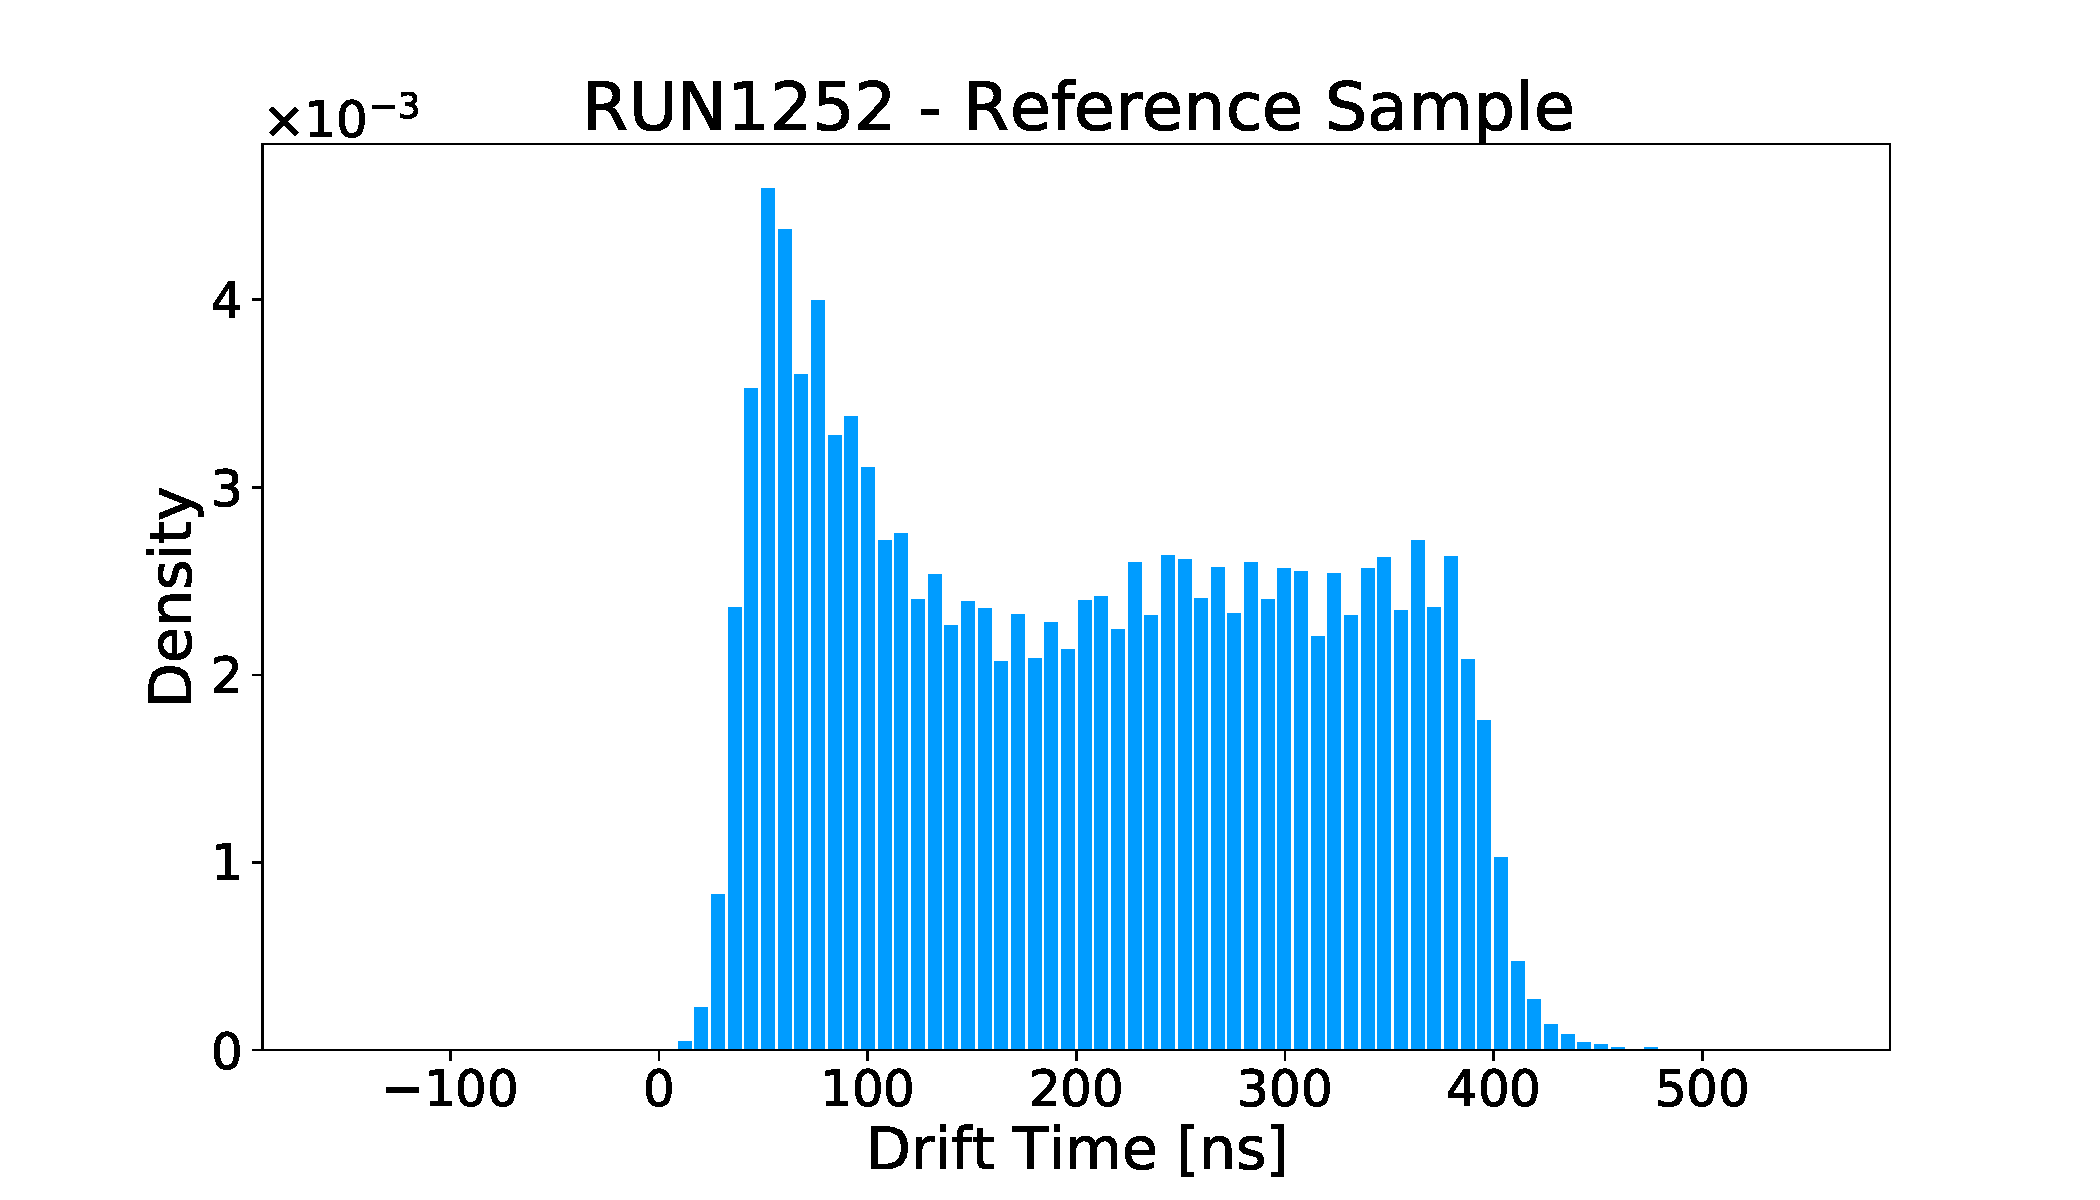
\includegraphics[width=1.0\textwidth]{./Images/results/reference.pdf} % \caption{Reference sample
    %     $\mathcal{N}_\R = 200000$} \label{fig:dt_ref:a} \end{subfigure}% \hfill \begin{subfigure}[b]{0.5\textwidth}
    %     \centering 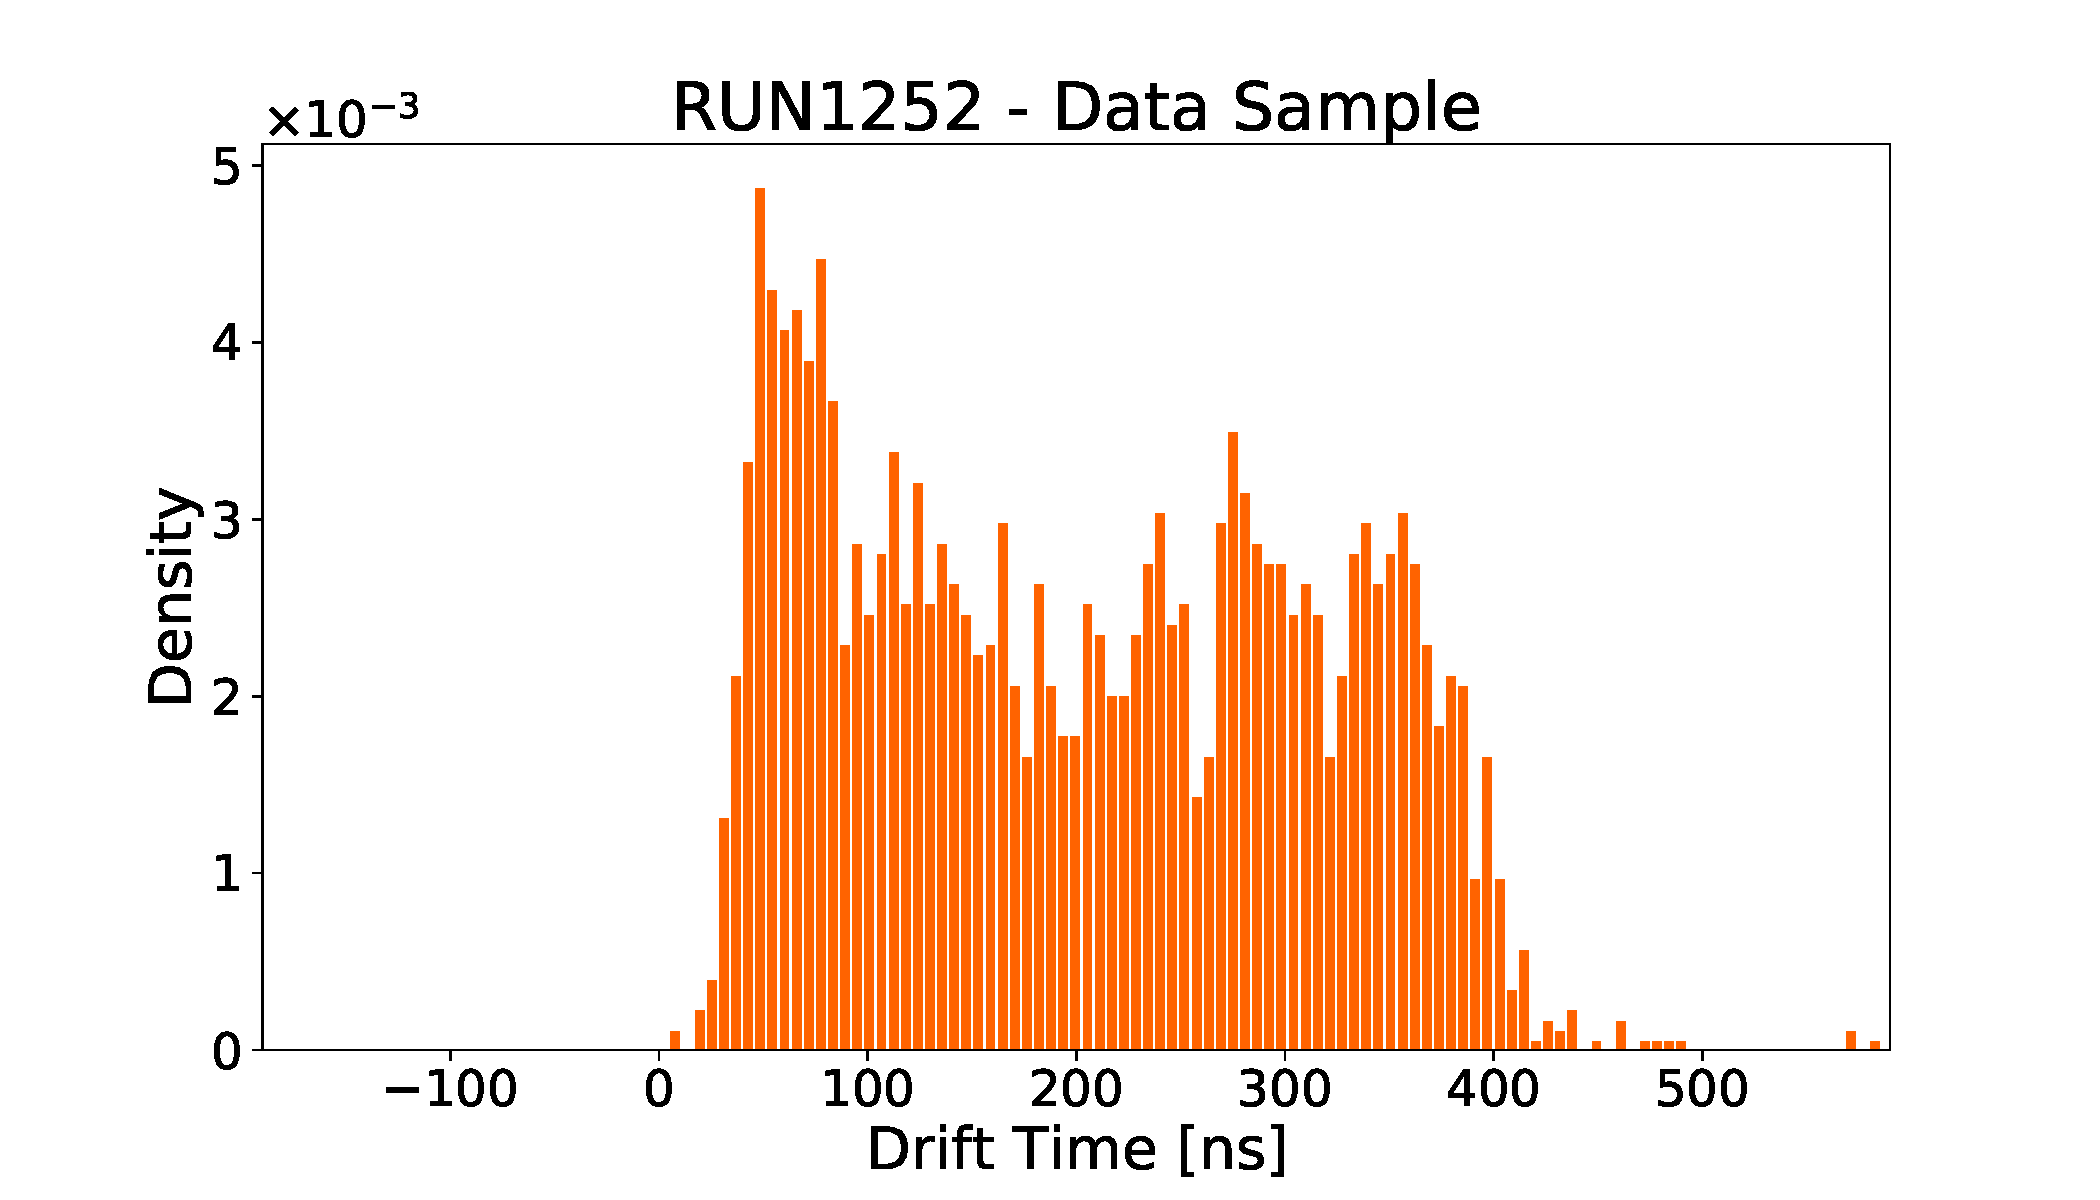
\includegraphics[width=1.0\textwidth]{./Images/results/sampled_ref.pdf} % \caption{Data sample
    %     $\mathcal{N}_\D = 3000$} \label{fig:dt_ref:b} \end{subfigure}%
    % \\
    \begin{subfigure}[b]{0.5\textwidth}
        \centering 
        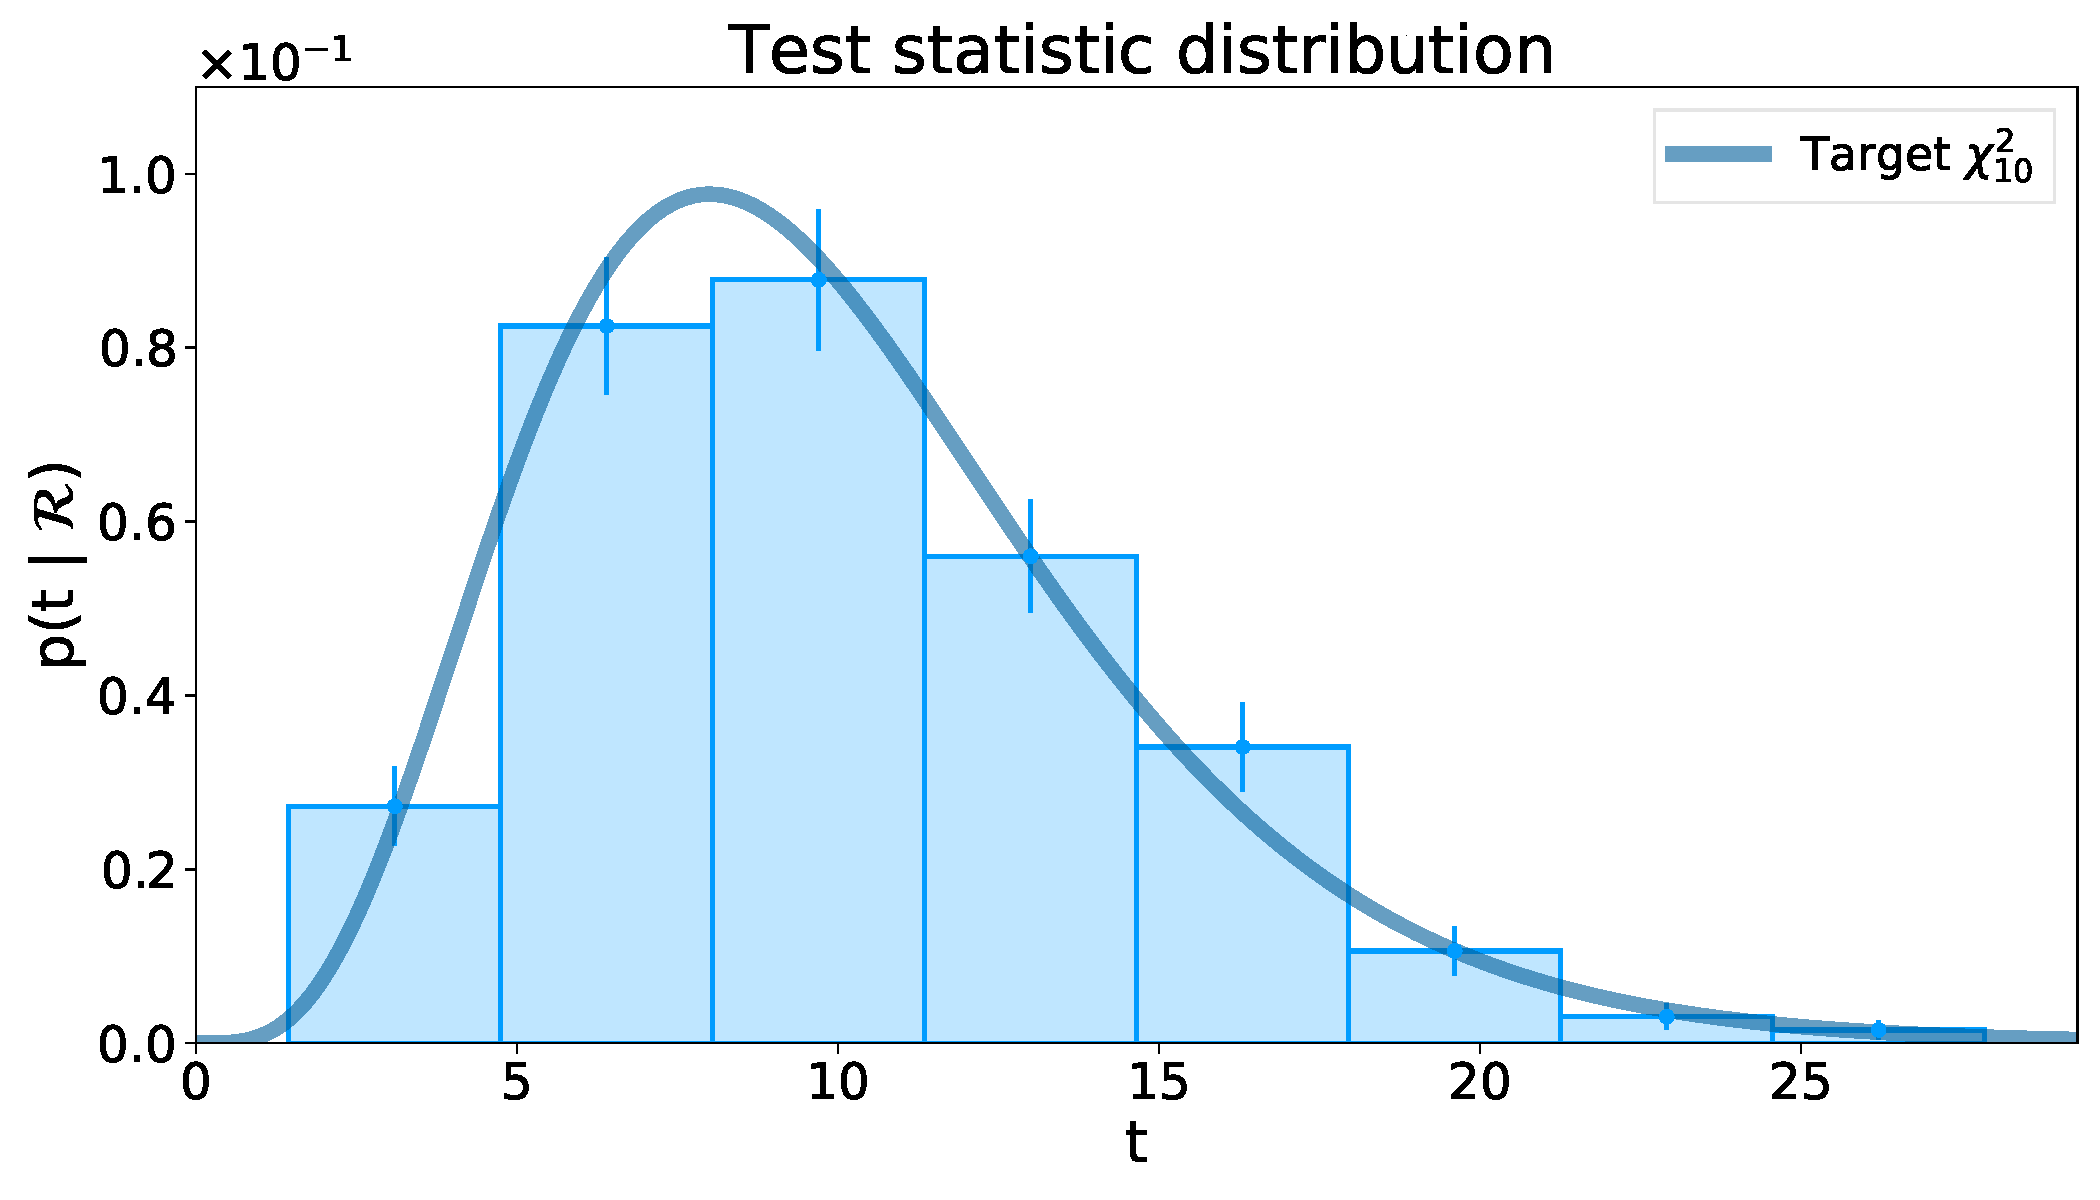
\includegraphics[width=1.0\textwidth]{../PLOTS/DRIFT_TIME/thesis/t_reference.pdf}
        \caption{Test statistic distribution with weight clipping $2.5$}
        \label{fig:dt_ref:c}
    \end{subfigure}%
    \begin{subfigure}[b]{0.5\textwidth}
        \centering 
        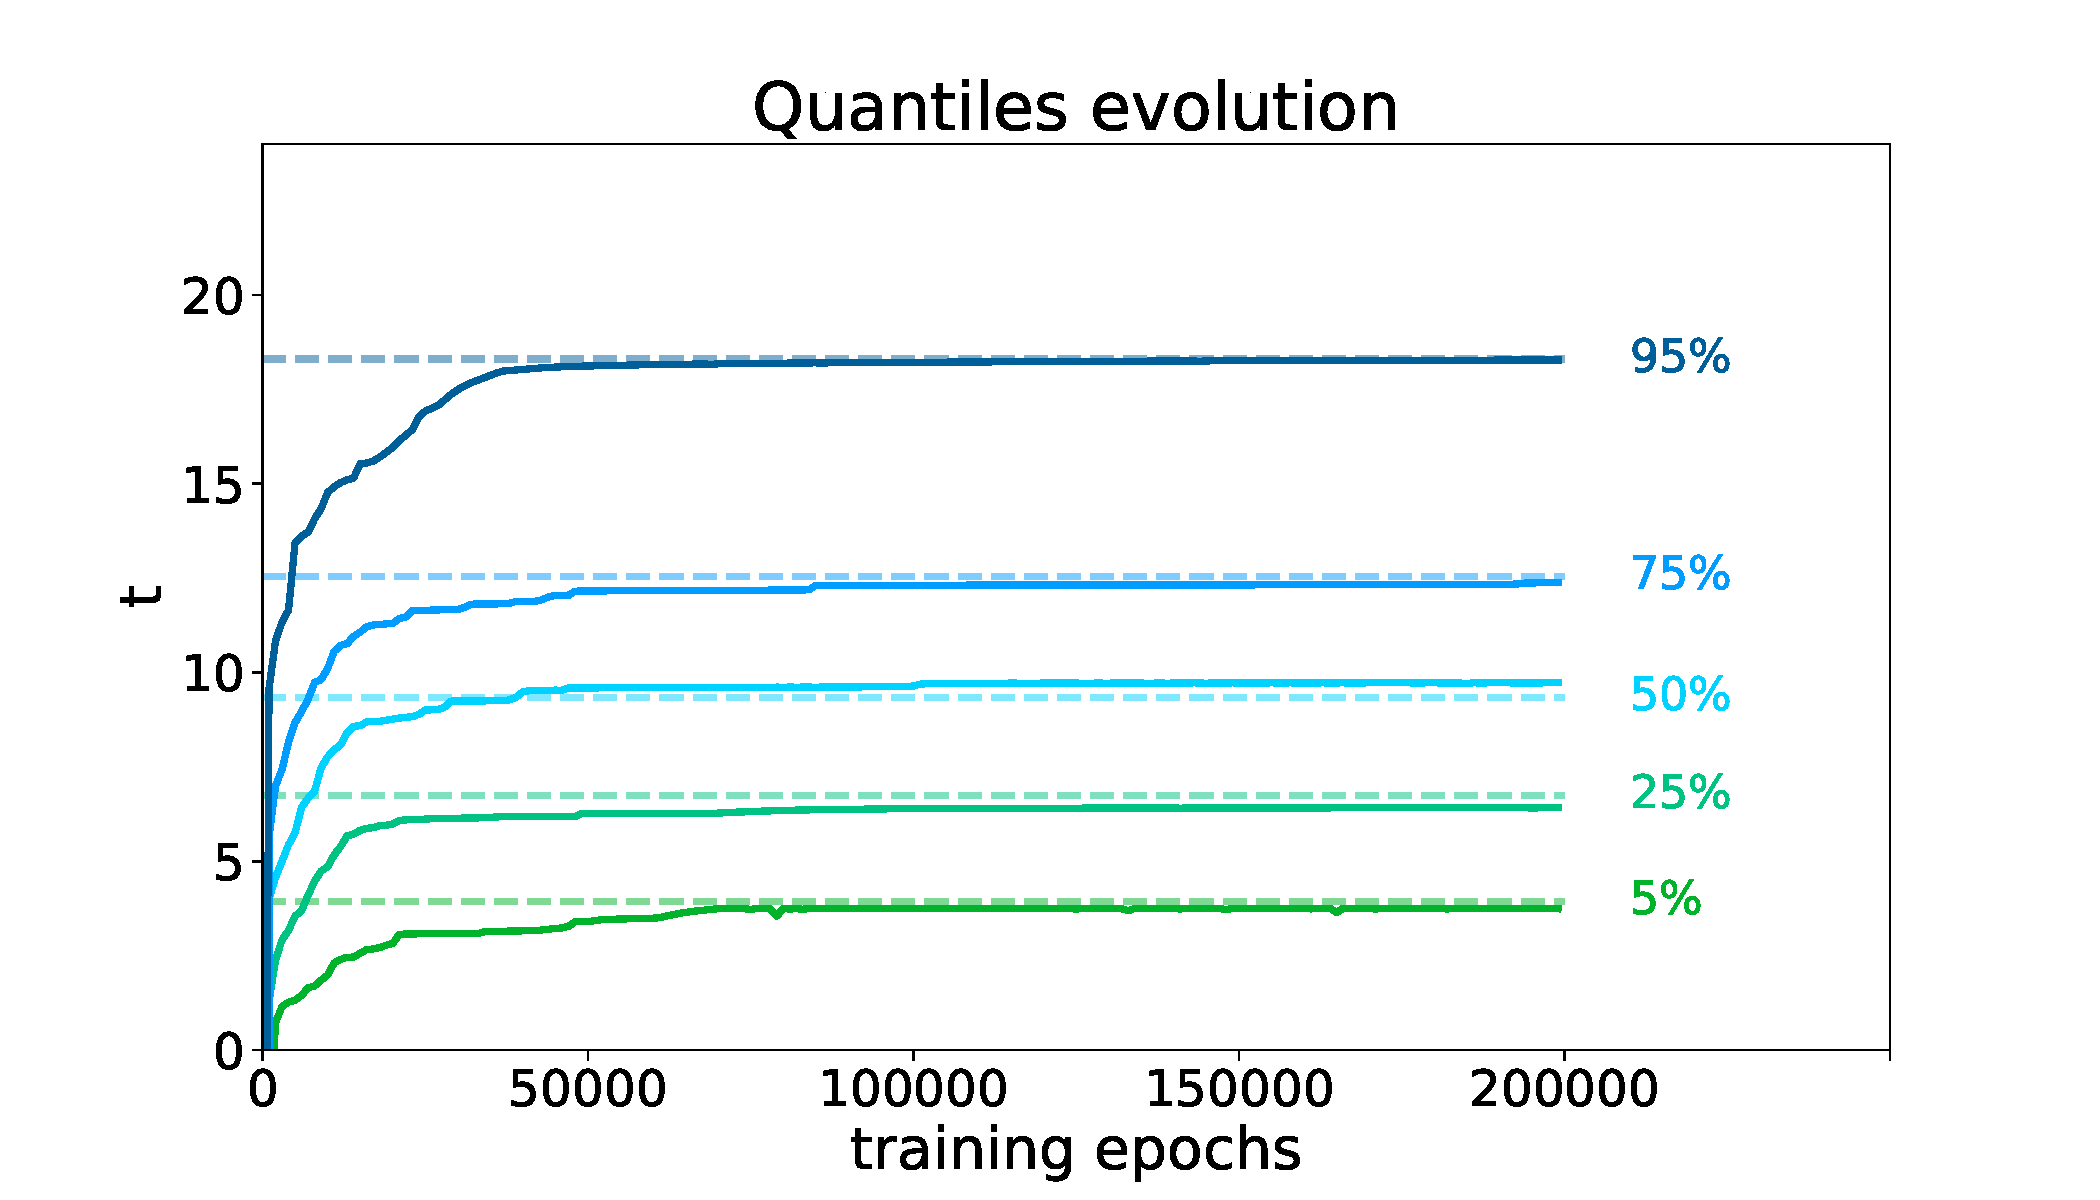
\includegraphics[width=1.0\textwidth]{../PLOTS/DRIFT_TIME/thesis/reference_quantiles.pdf}
        \caption{Quantiles evolution with weight clipping $2.5$}
        \label{fig:dt_ref:d}
    \end{subfigure}%
    \\
    \\
    \begin{subfigure}[b]{0.25\textwidth}
        \centering 
        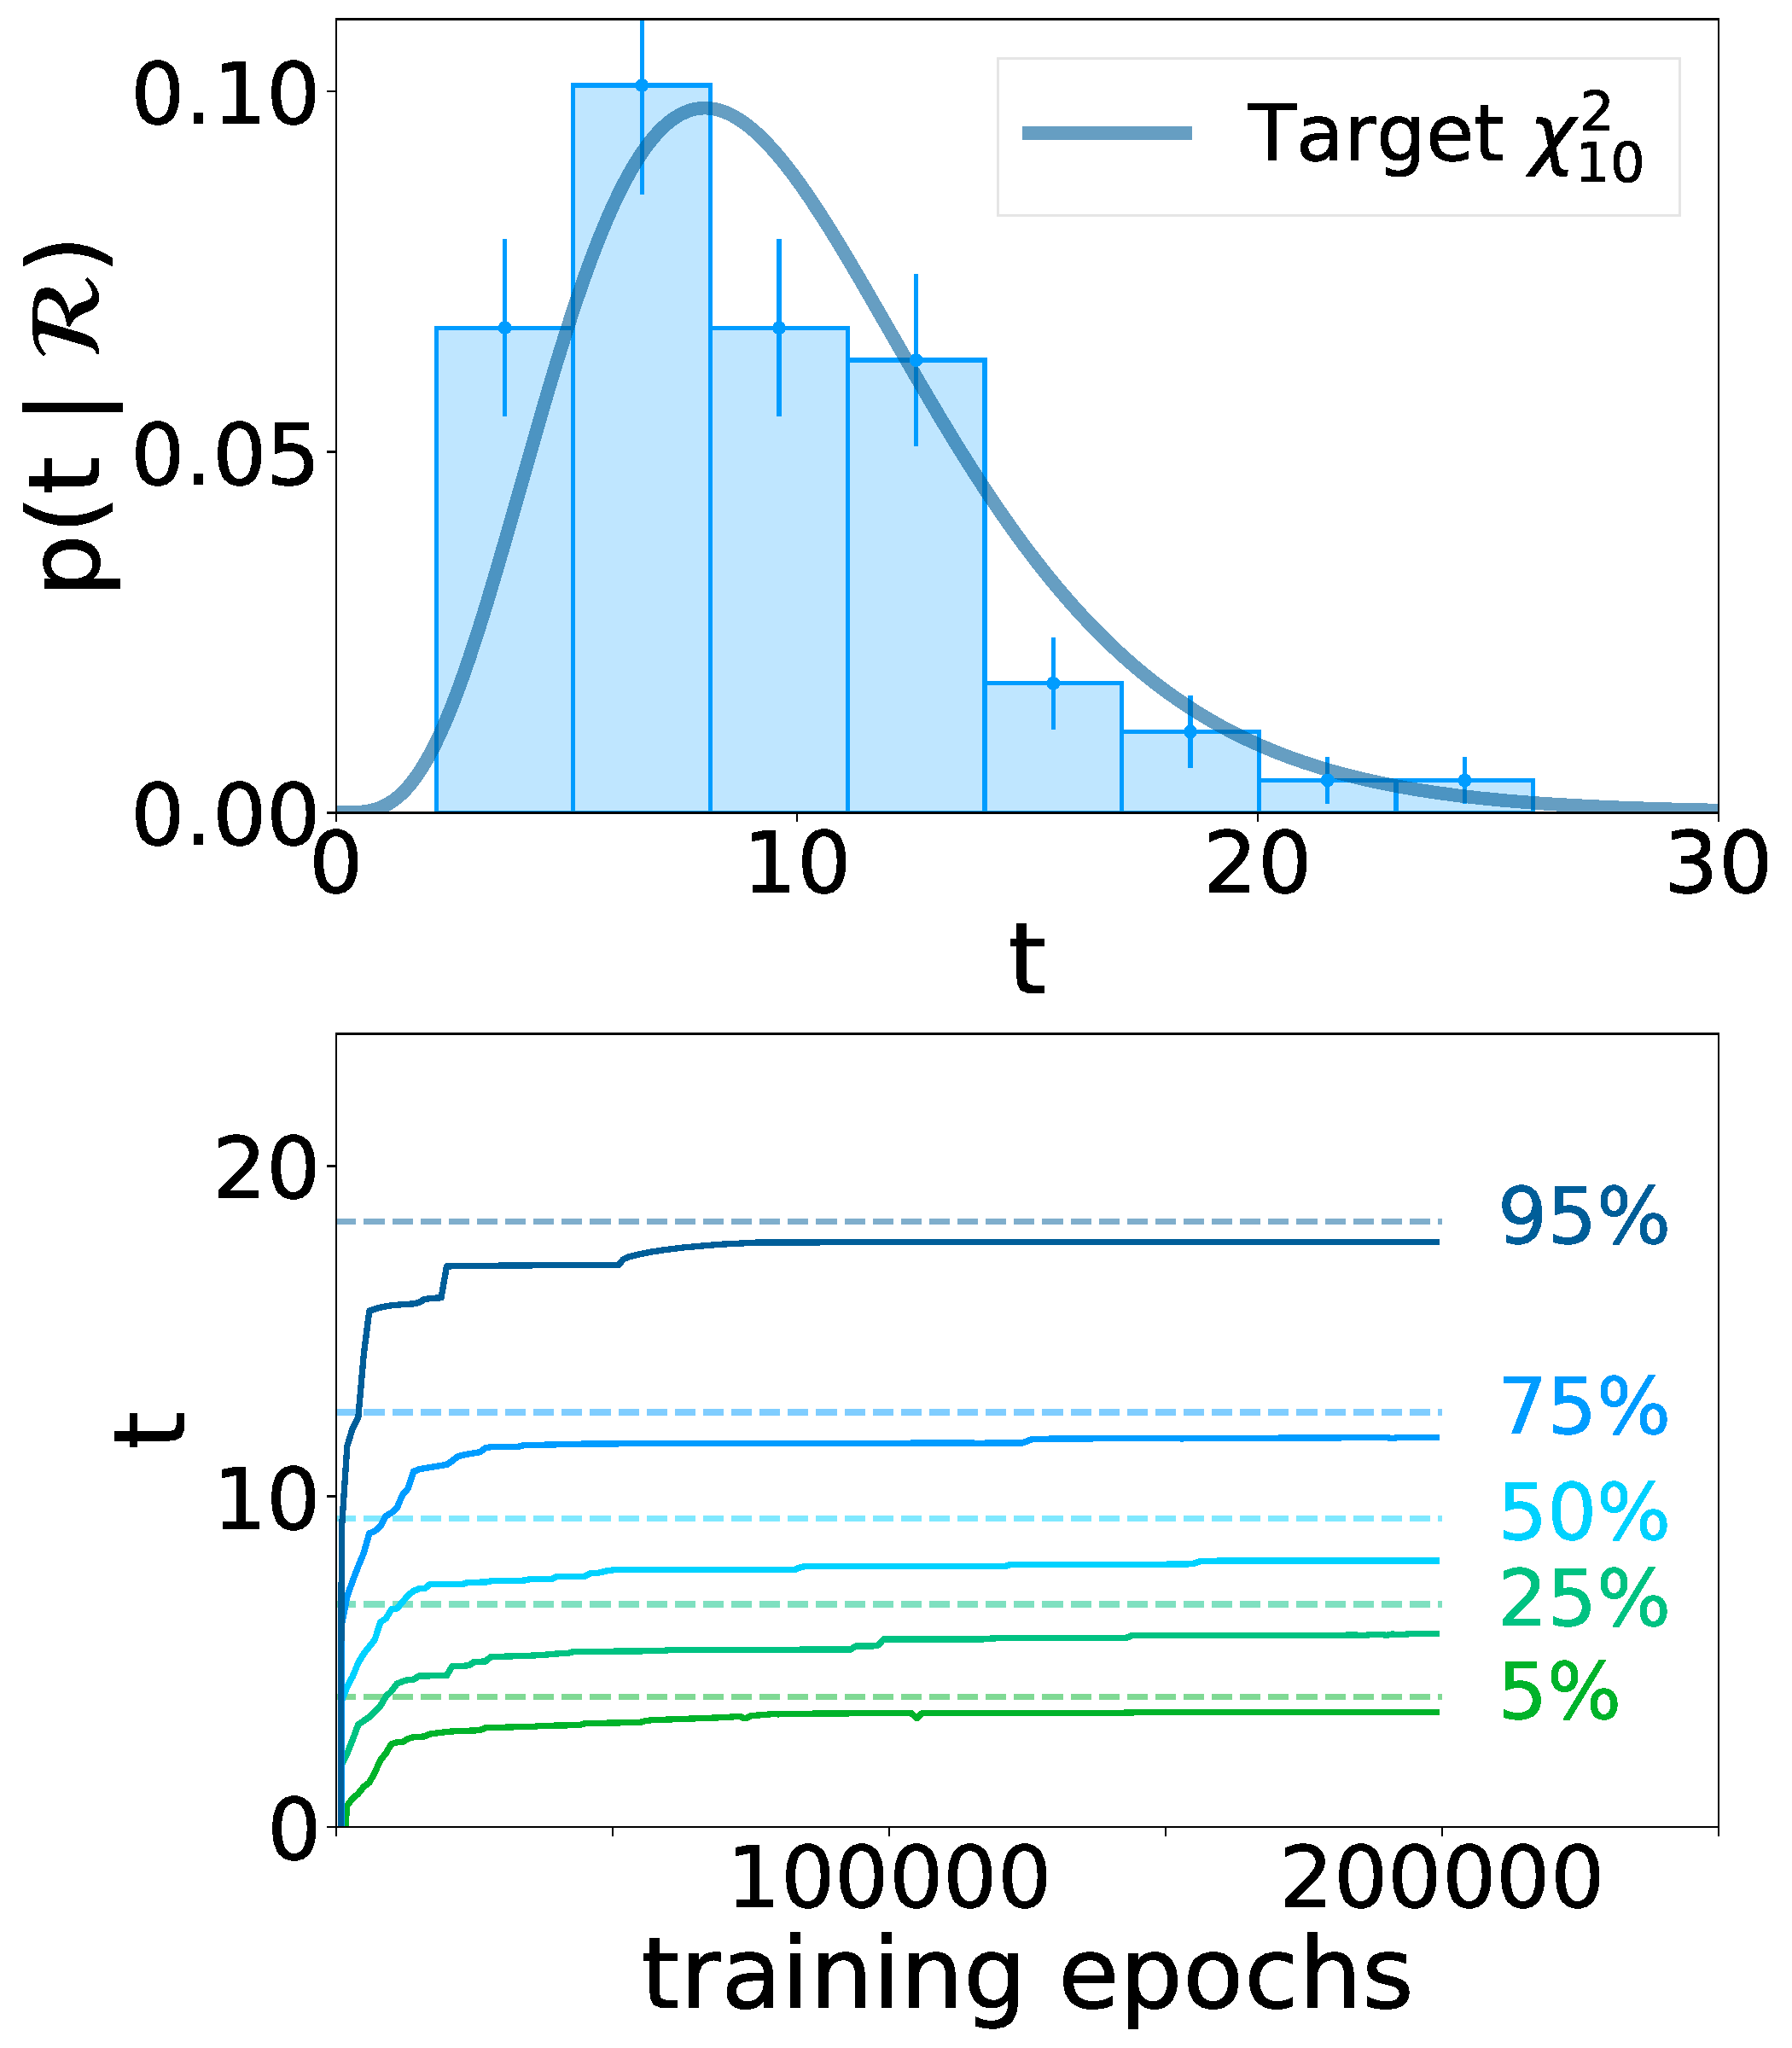
\includegraphics[width=1.0\textwidth]{../PLOTS/DRIFT_TIME/thesis/both_1_0.pdf}
        \caption{$W=1$}
        \label{fig:dt_ref:e}
    \end{subfigure}%
    \begin{subfigure}[b]{0.25\textwidth}
        \centering 
        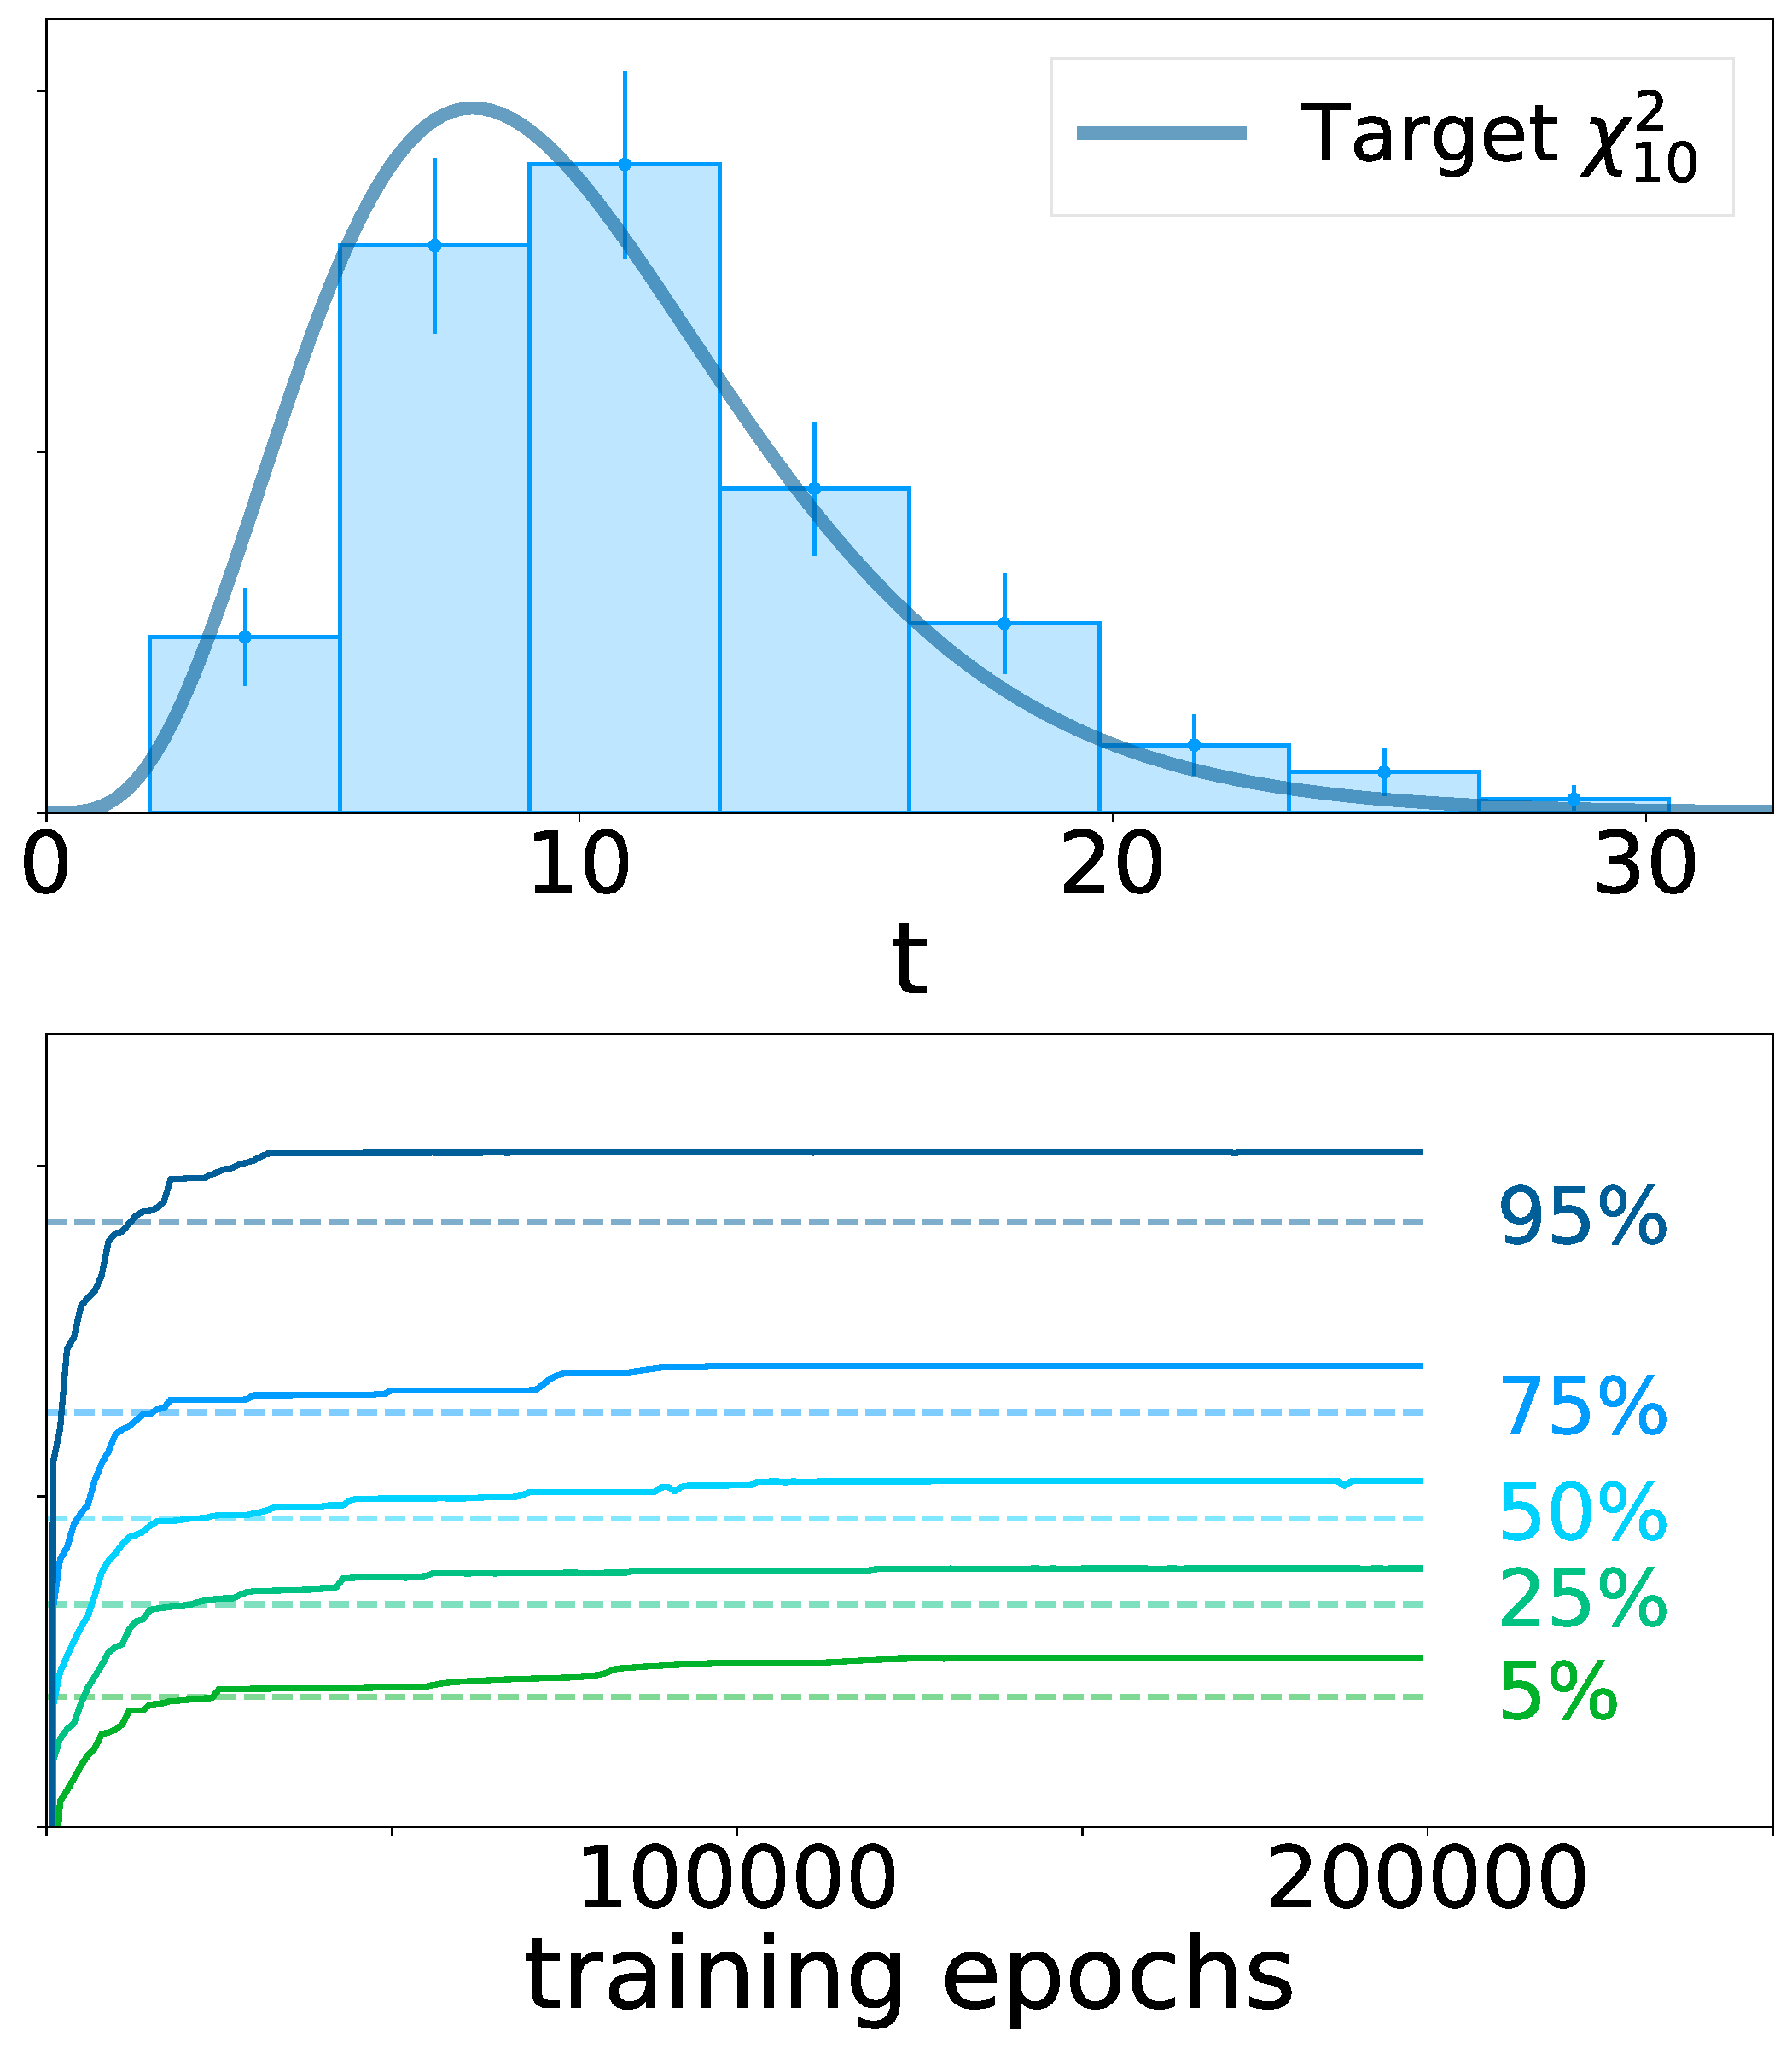
\includegraphics[width=1.0\textwidth]{../PLOTS/DRIFT_TIME/thesis/both_7_0.pdf}
        \caption{$W=10$}
        \label{fig:dt_ref:f}
    \end{subfigure}%
    \begin{subfigure}[b]{0.25\textwidth}
        \centering 
        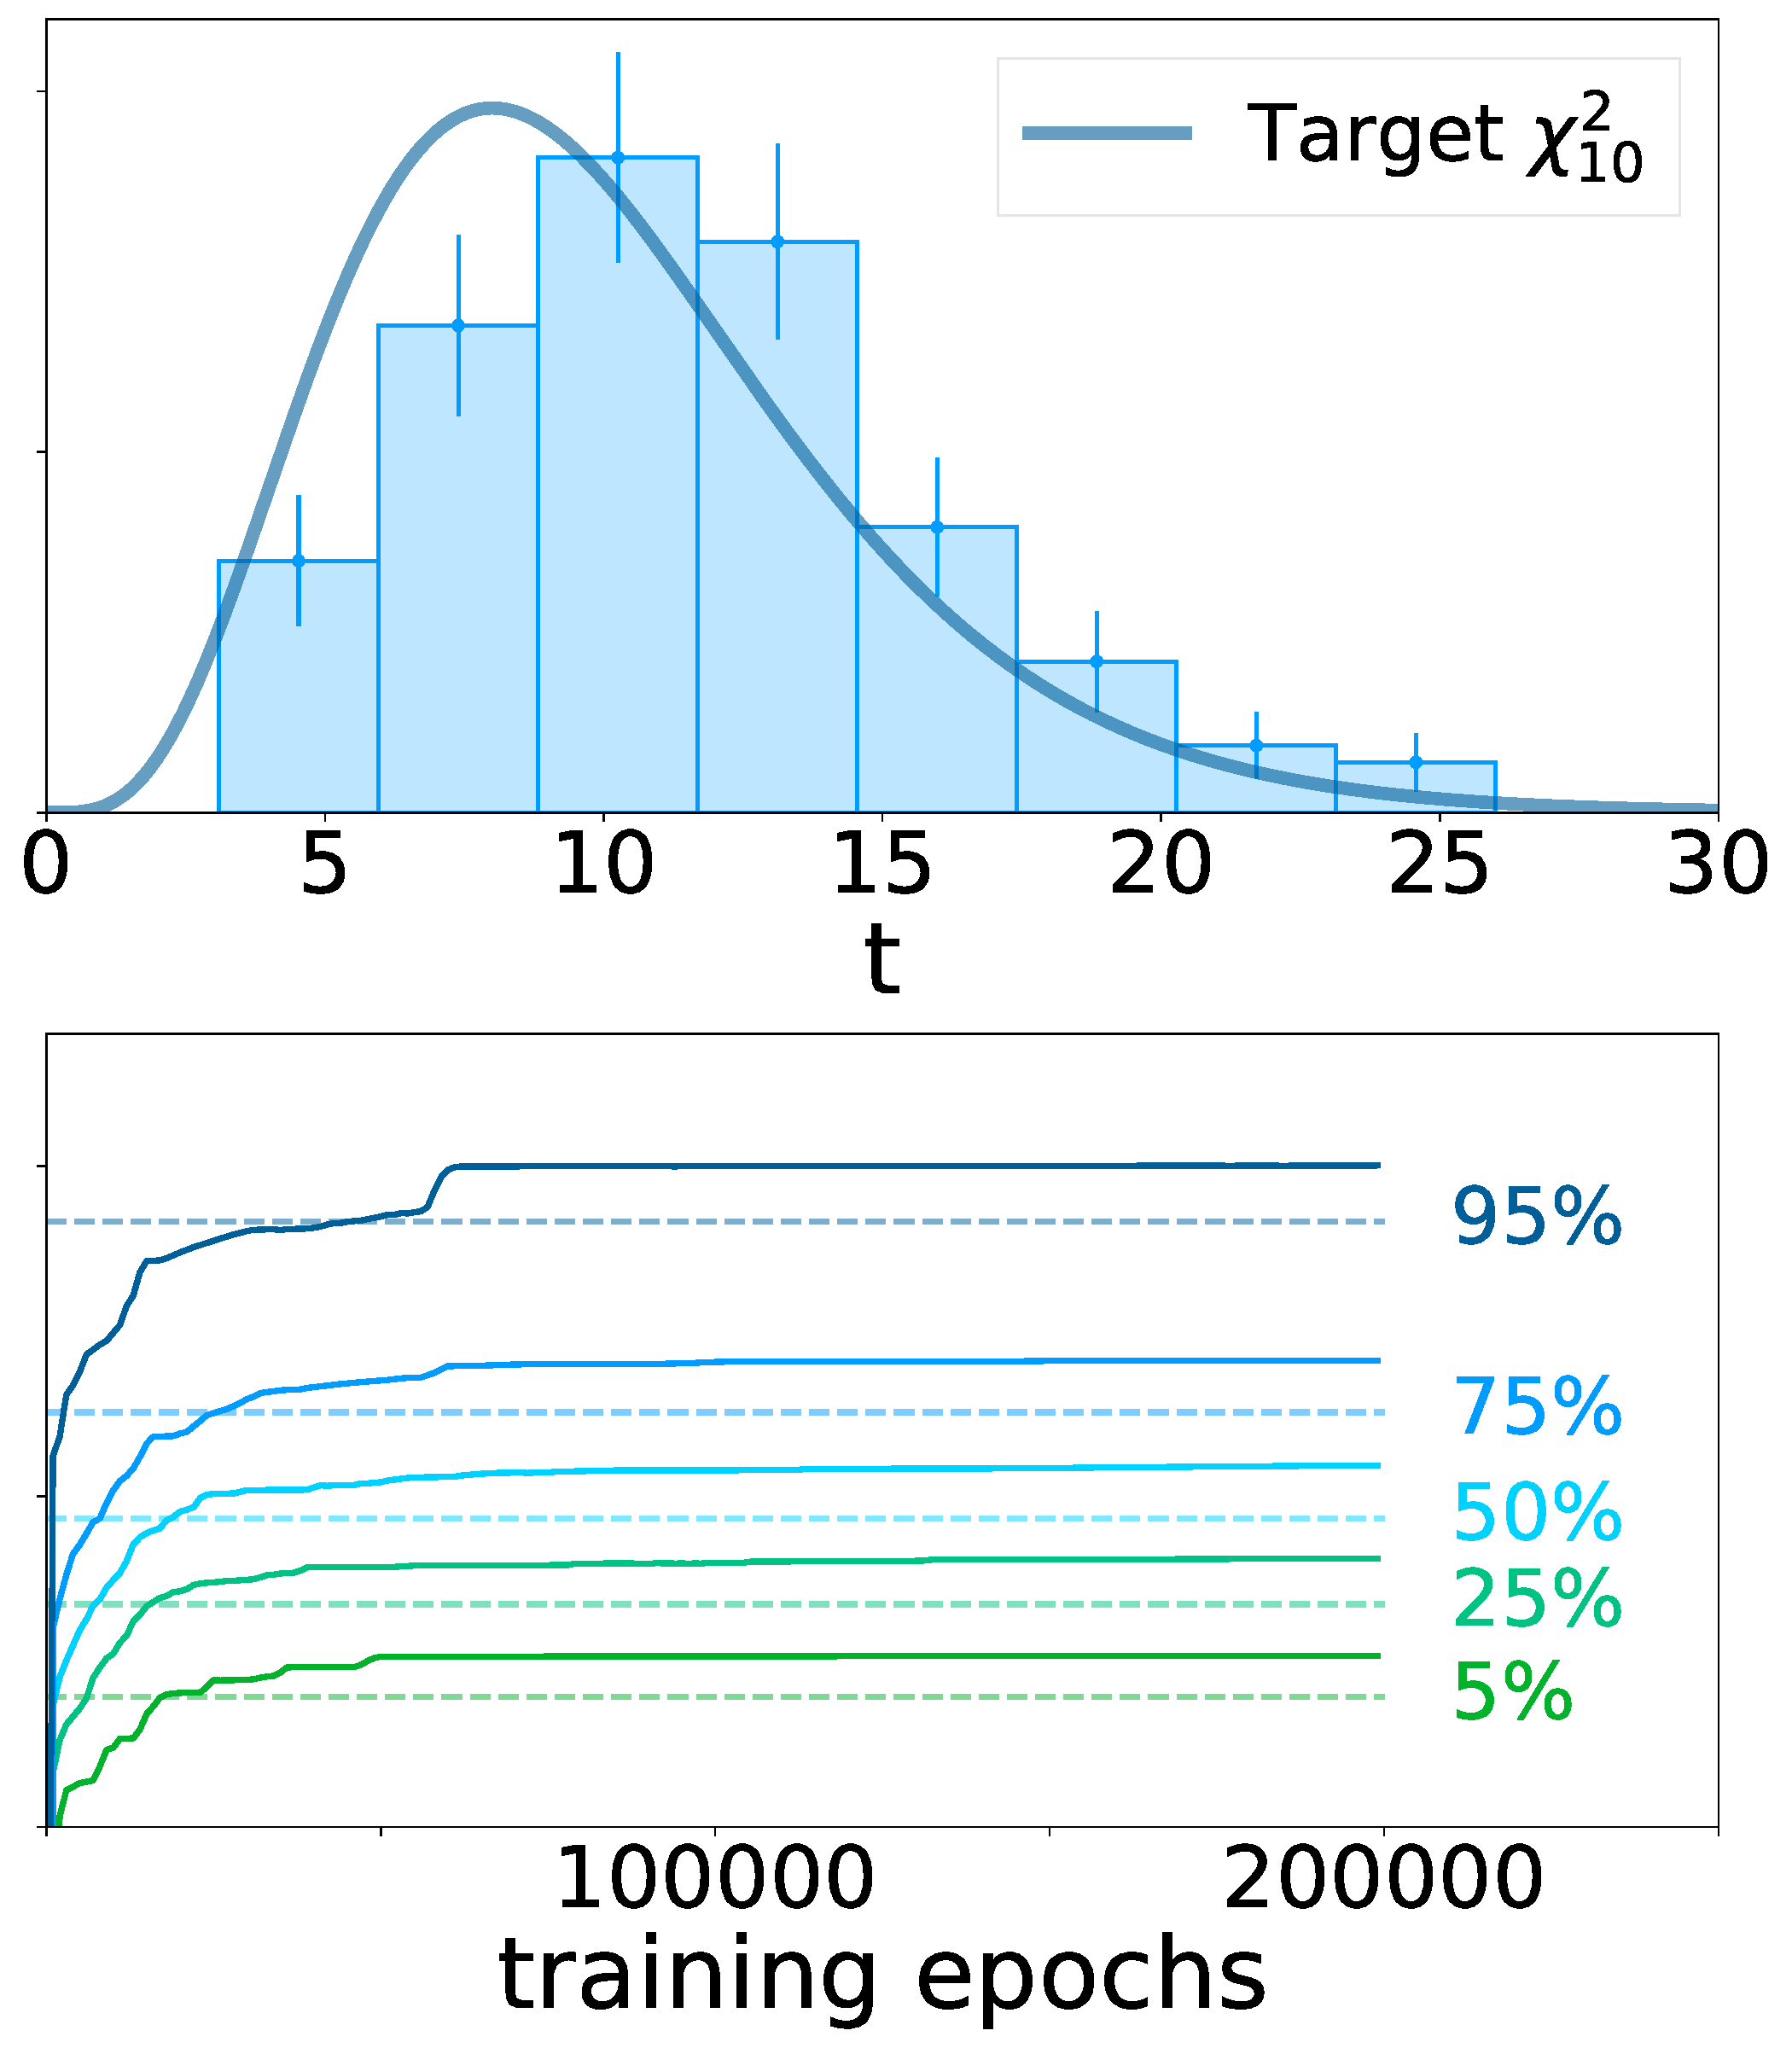
\includegraphics[width=1.0\textwidth]{../PLOTS/DRIFT_TIME/thesis/both_50_0.pdf}
        \caption{$W=50$}
        \label{fig:dt_ref:g}
    \end{subfigure}%
    \begin{subfigure}[b]{0.25\textwidth}
        \centering 
        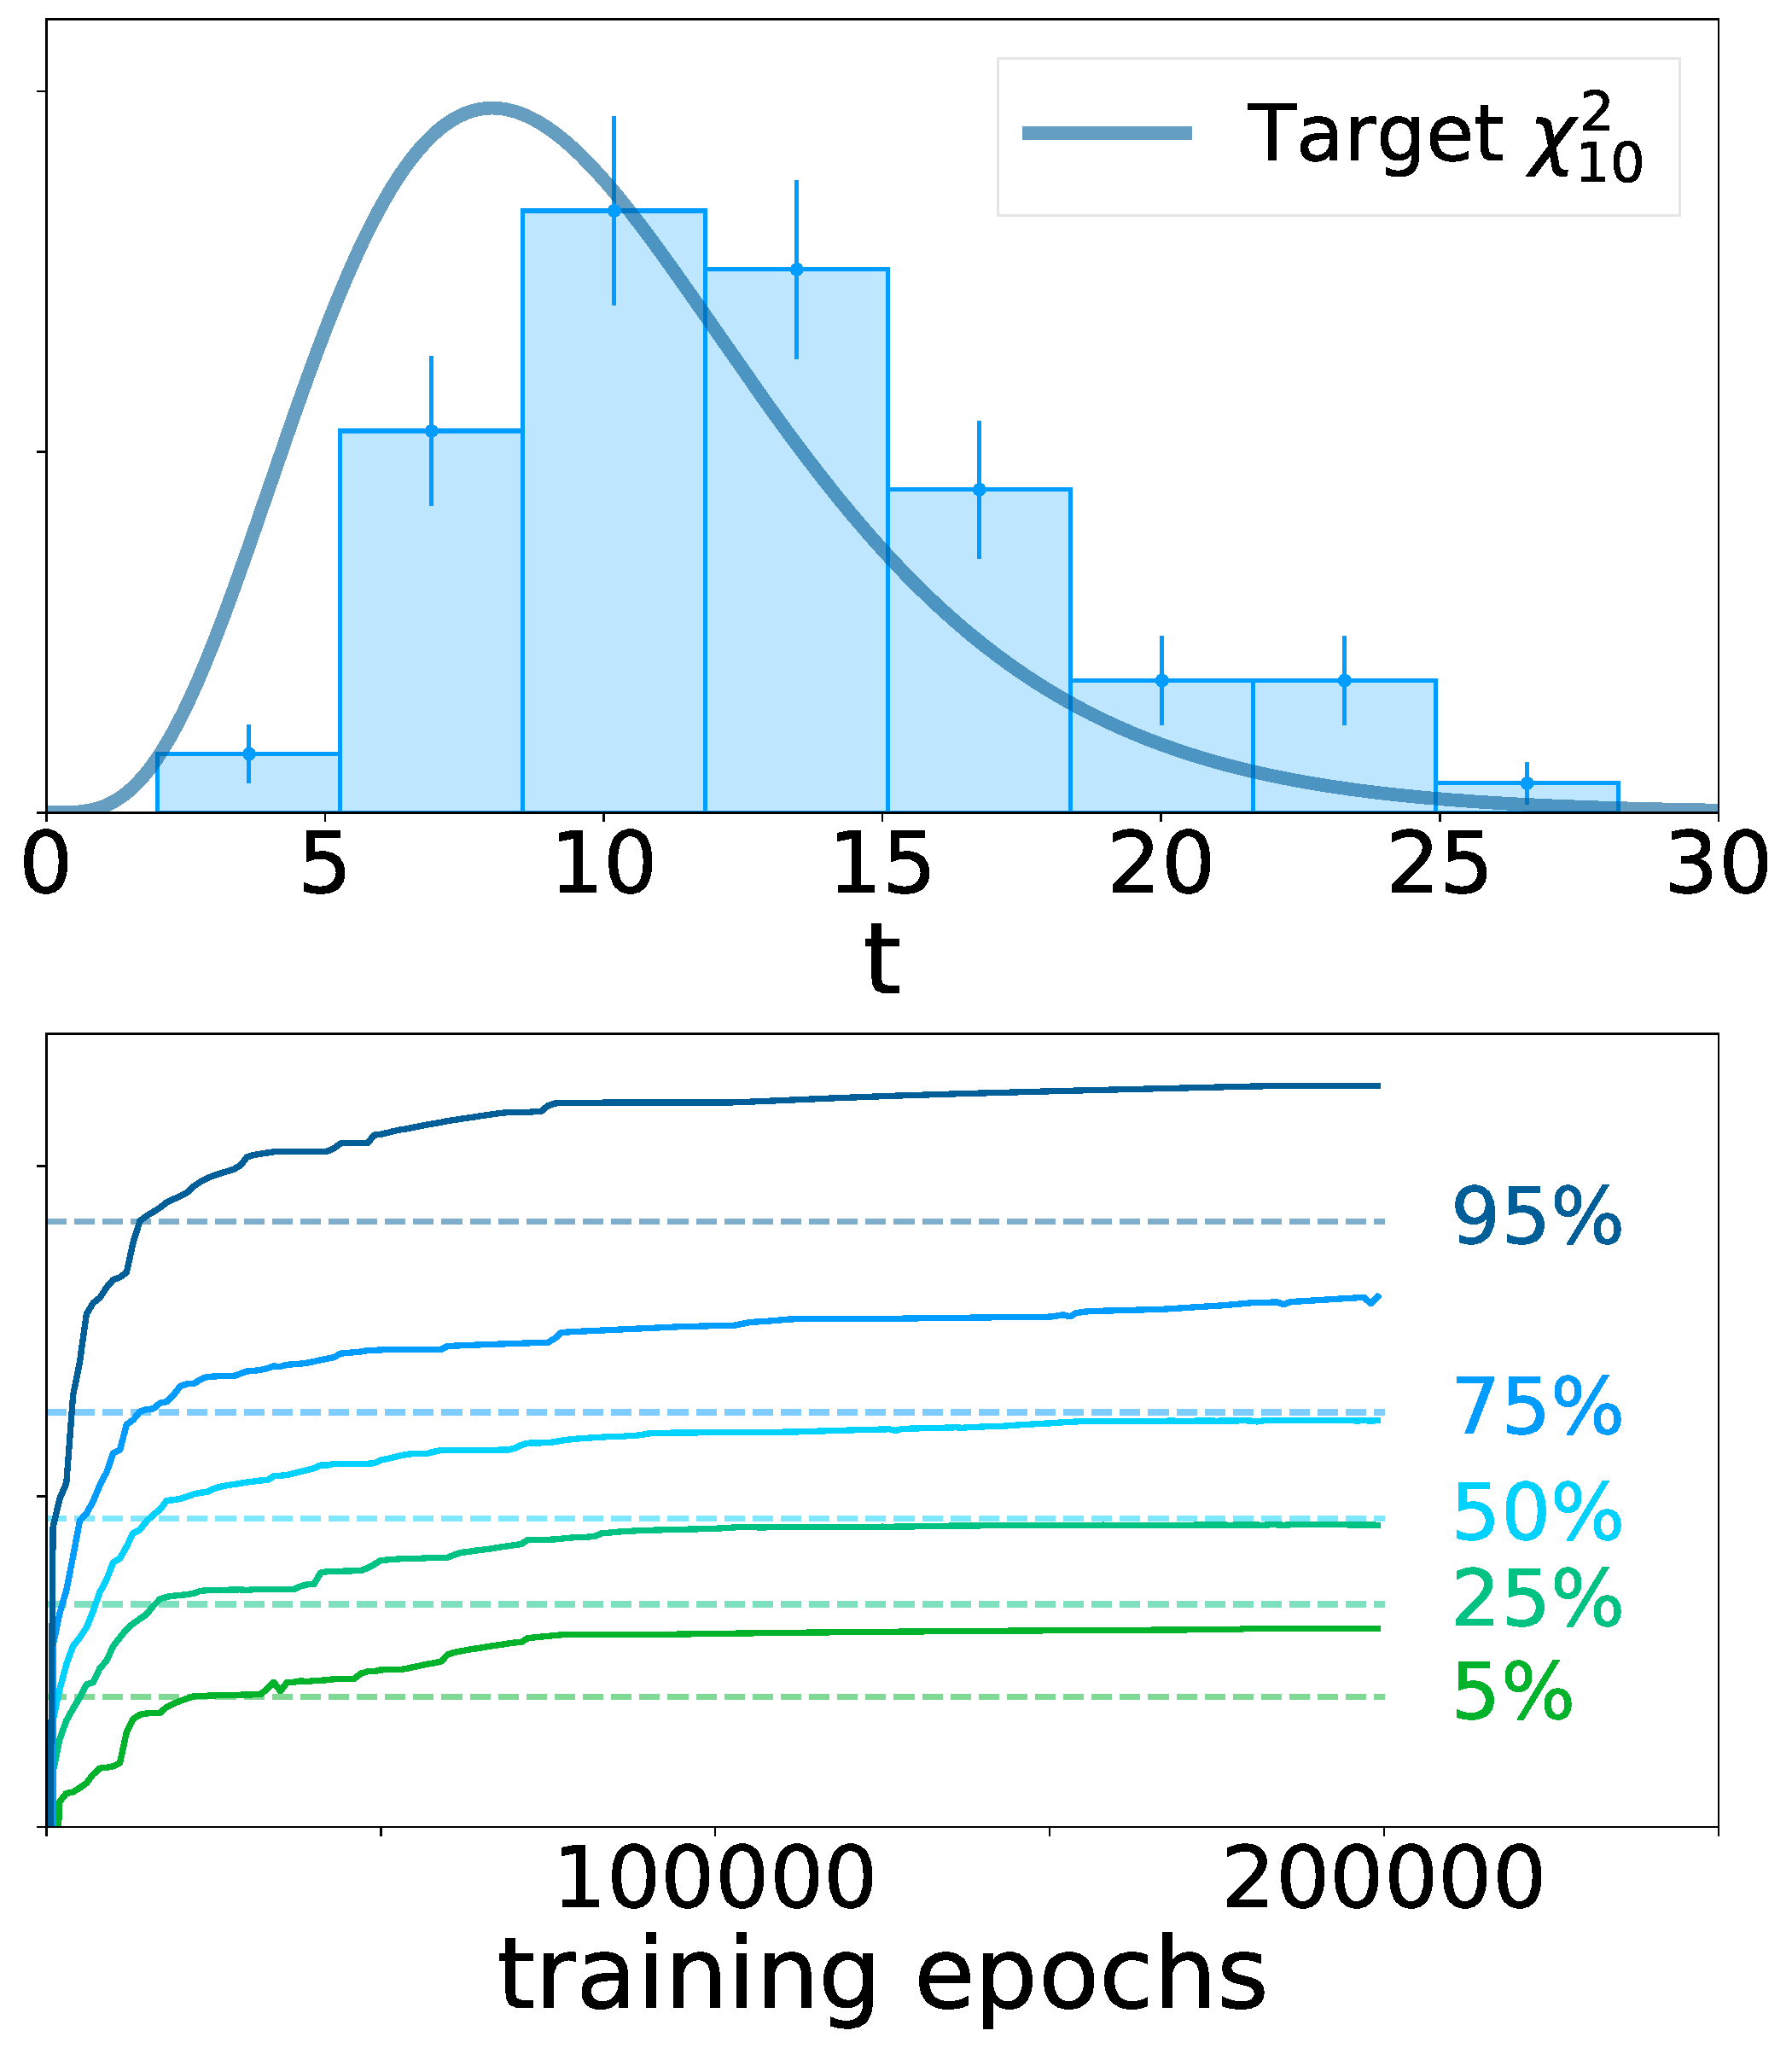
\includegraphics[width=1.0\textwidth]{../PLOTS/DRIFT_TIME/thesis/both_100_0.pdf}
        \caption{$W=100$}
        \label{fig:dt_ref:h}
    \end{subfigure}%
    \caption{Test statistic distributions after 200000 training epochs and evolution of their quantiles during the
    training process with an optimal weight clipping parameter (above) and other weight clipping values (below)}
    \label{fig:dt_ref}
\end{figure}

We see that for large values of the weight clipping $W$ (\autoref{fig:dt_ref:h}), the distribution looks shifted to the
right of the target $\chi^2$ with $10$ degrees of freedom. Moreover, the evolution of the quantiles tells us that the
training is not stable: the quantiles (especially the $95\%$ one) do not achieve a plateau. On the other hand, small
values of weight clipping (\autoref{fig:dt_ref:e}) make the distribution stable with training but slightly shifted
towards the left of the $\chi^2_{10}$ expectation. Instead, a good compatibility is obtained with a weight clipping
equal to $2.5$ (\autoref{fig:dt_ref:c} and \autoref{fig:dt_ref:d}): the quantiles reach a plateau near the quantiles of
the target $\chi^2_{10}$ and the distribution reproduces the $\chi^2_{10}$ formula quite accurately. 

The first strategy that we have implemented to search for the optimal weight clipping parameter is thus the following:

\begin{itemize}
    \item Starting from a large value of $W$ (in our case $W=100$) decrease it until the $95\%$ quantiles reaches a
    plateau as a function of the training epochs (in our case $W_{\text{max}}=50$ in \autoref{fig:dt_ref:g}).
    \item In the range of weight clippings below $W_{\text{max}}$ (where the plateau is always reached) choose the
    largest $W$ that also gives the highest compatibility between $p(t\,|\,\R)$ and $\chi^2_{10}$.
\end{itemize}

It is essential to set the weight clipping parameter as large as possible to maximize the expressive power of the
network. However, a refined strategy has been applied to reduce the computational burden of the above search for $W$: 

\begin{itemize}
    \item Starting from a large and a small value of $W$ (in our case $W=100$ and $W=1$), train the network on a limited
    number of $\D_\R$ datasets ($40$ for example).
    \item Compute the median of the $p(t\,|\,\R)$ distribution: it will be above the median of the target $\chi^2_{10}$
    distribution for the large value of $W$ and below the median of the target $\chi^2_{10}$ distribution for the small
    value of $W$.
    \item In the window of weight clippings that produce a $p(t\,|\,\R)$ distribution with median similar to the
    $\chi^2_{10}$ one, replicate the first two bullet points using a larger number of $\D_\R$ datasets ($150$ for
    example).
    \item Employ a compatibility test to pick up the optimal weight clipping value inside the window. In our case, we
    have chosen to perform a Kolmogorov-Smirnov (KS) test and maximized (in the window of optimal weight clippings) the
    $p$-value for the compatibility between the $p(t\,|\,\R)$ distribution and the target $\chi^2_{10}$.
    \item Consider using an even larger amount of  $\D_\R$ datasets ($400$ in our case) to ultimately test the validity
    of the S. Wilks result and obtain a KS $p$-value above a given threshold.
\end{itemize}

Note that this refined strategy, even though not explicitly, finds the largest $W$ that leads to a $95\%$ quantile
plateau and maximizes the compatibility between the distributions.

To ultimately maximize the expressive power of the network, more complex architectures should be explored. However, as
reported in \cite{zanetti}, complexity cannot be increased indefinitely: too complex architectures cannot be made
compatible with the $\chi^2_{\nu}$ for any choice of the weight clipping parameter. Moreover, employing an overly
complicated neural network could be self-defeating for our data quality monitoring tasks, as it would increase the
algorithm's run time even more. In addition to that, since we are dealing with mono-dimensional datasets, it is not
strictly necessary to employ the most powerful tools at our disposal. 


\section{Algorithm performance on DQM tasks}

With the tuned hyperparameters of the network, we are ready to test the algorithm on real data quality monitoring
scenarios. Referring to \autoref{fig:dt_cat}, we've already stated that RUN1252 (\autoref{fig:dt_cat:a}) is our
reference run. Thus, we sampled a $\mathcal{N}_\R = 200000$ reference dataset from the whole run. Then, instead of
sub-sampling from the same run as we have done for the hyperparameters tuning session, we sampled a single dataset of
$\mathcal{N}_\D = 3000$ from a different run. It is key to stick with the same number of events in $\R$ and $\D$ chosen
to tune the network, as the weight clipping parameter heavily depends on such conditions. Namely, if we want to change
$\mathcal{N}_\R$ and $\mathcal{N}_\D$ at some point in the process, we would need to tune the network again using $\R$
and $\D_\R$ datasets having the new $\mathcal{N}_\R$ and $\mathcal{N}_\D$ events. \\ 

Referring again to \autoref{fig:dt_cat}, we sampled a $\mathcal{N}_\D = 3000$ dataset from each of the three remaining
distributions (namely RUN1253, RUN1265 and RUN1242). As mentioned in \autoref{sec:exp_timebox}, those three runs fall
into three different categories. Precisely,  RUN1253 (\autoref{fig:dt_cat:b}) is a \textit{good} run, almost identical
to our reference run: we would expect that our algorithm do not detect any discrepancy between $\D_{1253}$ and $\R$. In
other words, the observed test statistic $t_{\text{obs}}$ resulting from the training process should fall somewhere near
the median of the $\chi^2_{10}$ distribution. On the other hand, RUN1265 (\autoref{fig:dt_cat:c}) is a
\textit{discrepant} run and our expectations are that the algorithm would notice a sensible deviation in $\D_{1265}$
with respect to $\R$. Thus, the output $t_{\text{obs}}$ should fall somewhere in the right-hand tail of the
$\chi^2_{10}$ distribution. Finally, RUN1242 (\autoref{fig:dt_cat:d}) is a \textit{bad} run and, if the network is
correctly learning, the $t_{\text{obs}}$ in this case should be larger than the previous one, as the discrepancy between
$\D_{1242}$ and $\R$ is more pronounced. The observed test statistics $t_{\text{obs}}$ for each of the three tested runs
after the training process are shown in \autoref{fig:t_obs}. 


%grafici
\begin{figure}[t]
    \centering
    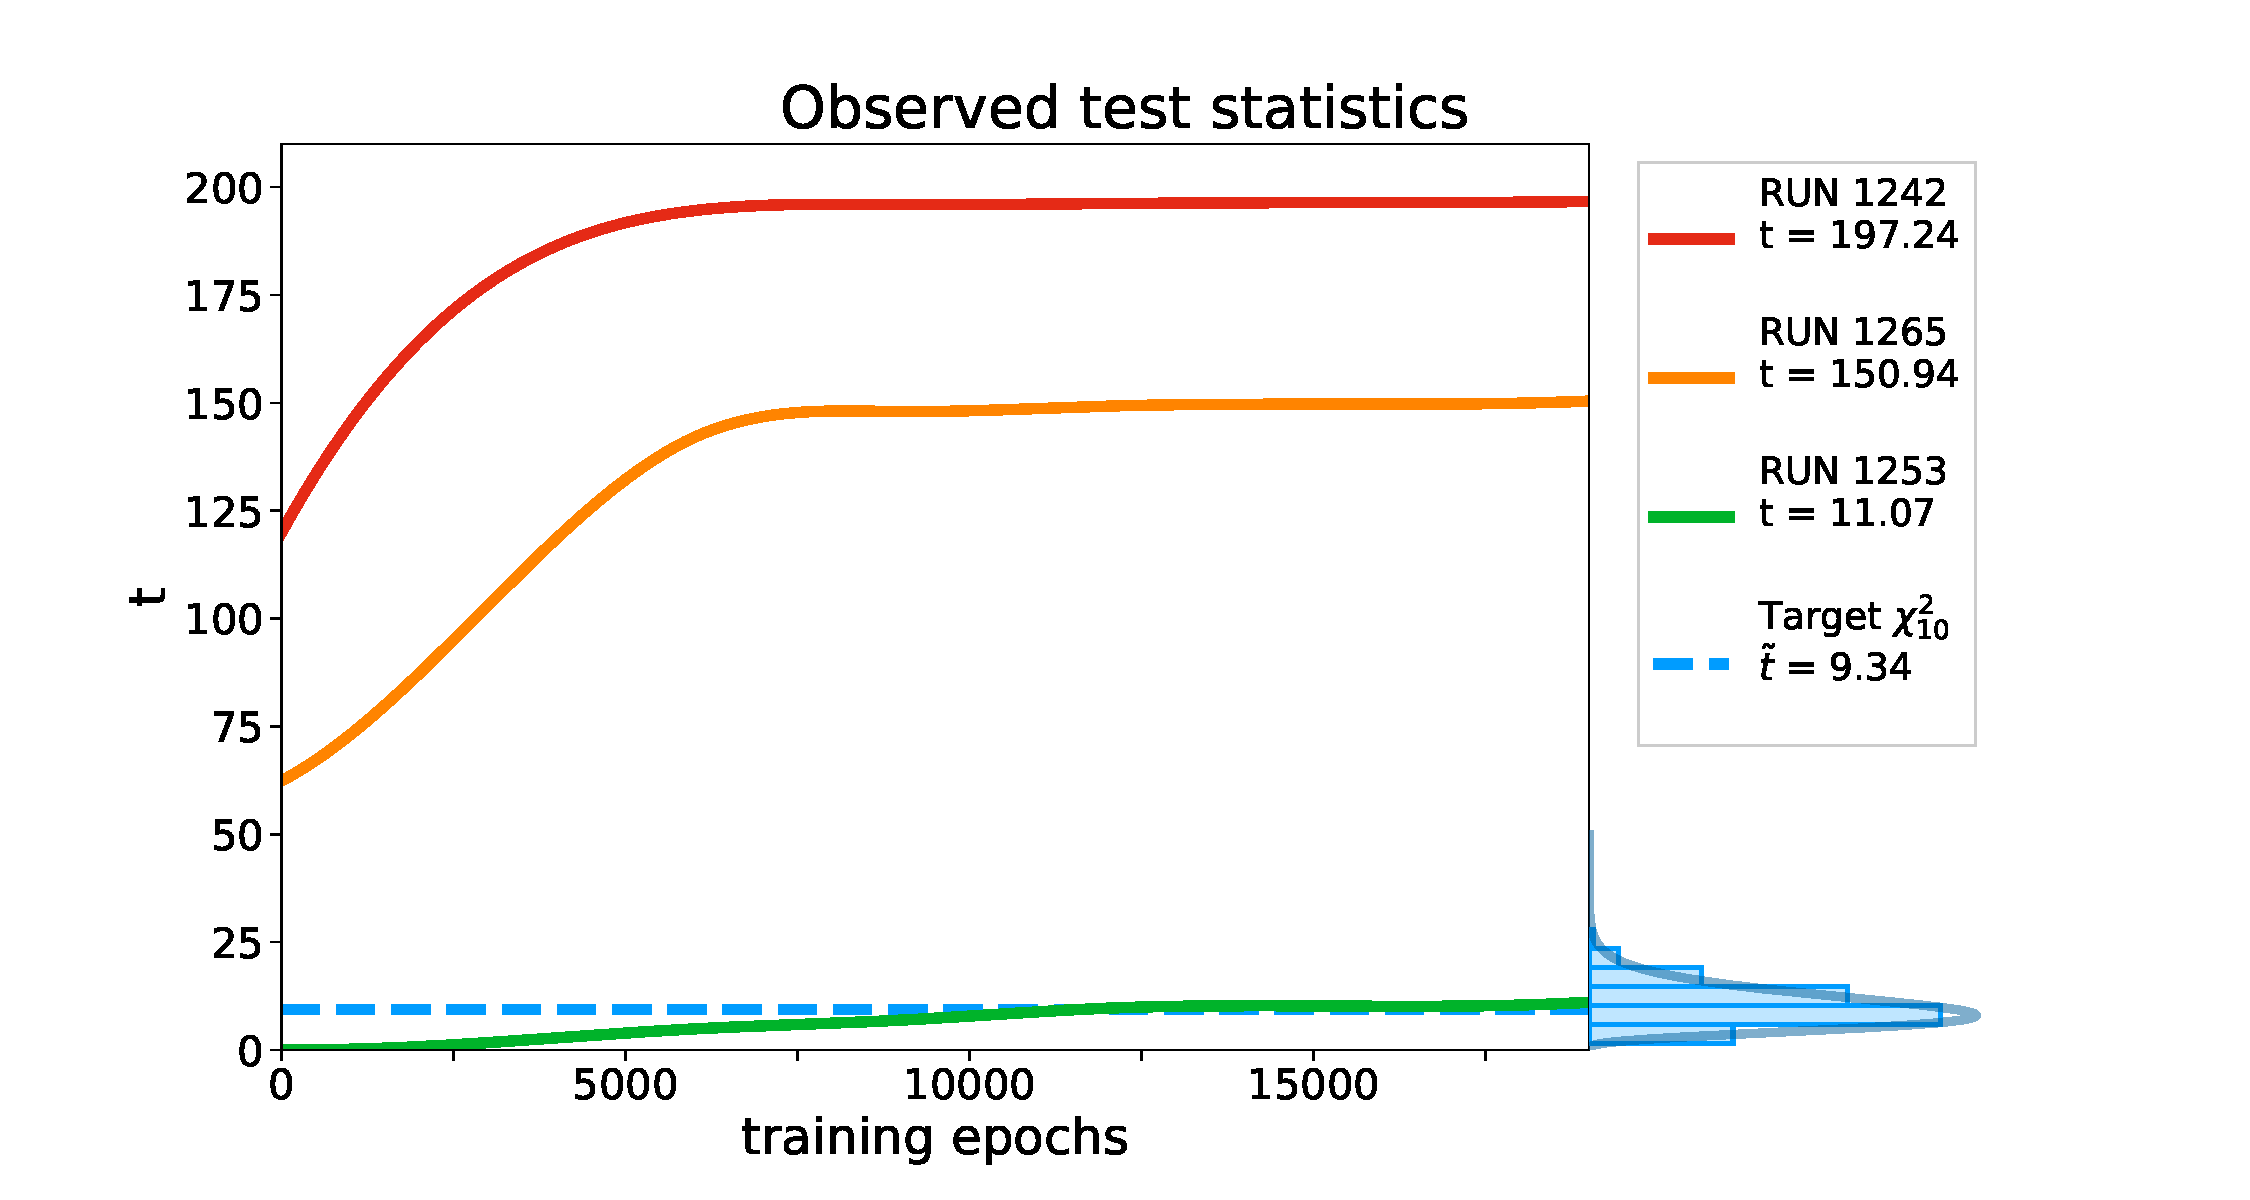
\includegraphics[width=0.8\textwidth]{../PLOTS/DRIFT_TIME/thesis/t_all_advanced.pdf}
    \caption{Evolution of the $t_{\text{obs}}$ during the training process for each of the three tested runs}
    \label{fig:t_obs}
\end{figure}

Starting from below, we find that $t_{\text{obs}}^{1253}$ falls right under the target $\chi^2_{10}$ distribution, close
to its median $\tilde{t}$. This outcome indicates that the algorithm cannot detect any deviation from $\R$ in
$\D_{1253}$ and treats the latter as a reference sub-sample following the null hypothesis. On the other hand,
$t_{\text{obs}}^{1265}$ and $t_{\text{obs}}^{1242}$ are consistently above the target $\chi^2_{10}$ median $\tilde{t}$:
the neural network thus found discrepant data in both $\D_{1265}$ and $\D_{1242}$. Furthermore, having
$t_{\text{obs}}^{1242}$ sensibly larger than $t_{\text{obs}}^{1265}$ shows that the algorithm found $\D_{1242}$ more
discrepant than $\D_{1265}$. Finally, note that a few thousands of training epochs are sufficient to reach a plateau and
have a stable $t_{\text{obs}}$ value. The exact agreement between our predictions and the actual algorithm performance
is a great success. It means that the procedure is working as expected, and the algorithm behavior is under control. 

\subsection{Discrepancy assessment}\label{sec:disc_ass}

We have already stated in \autoref{sec:overview} that we intended to quantify the probability that a discrepancy is
present in $\D$ by comparing $t_{\text{obs}}$ with the $p(t\,|\,\mathbfcal{R})$ distribution. In \autoref{eq:pval} we
have introduced the observed \textit{p}-value and its corresponding significance $Z(p)$. However,
$t_{\text{obs}}^{1265}$ and $t_{\text{obs}}^{1242}$ locate too far on the right-hand tail of the distribution and
\autoref{eq:pval} cannot return a non-zero \textit{p}-value. Hence, we have tried to exploit the approximation 

\begin{equation}\label{eq:pval_approx}
    p_{\text{obs}} =
    \int_{t_{\text{obs}}}^{+\infty}p(t\,|\,\mathbfcal{R})\,\text{d}t
    \simeq
    \int_{t_{\text{obs}}}^{+\infty}\chi^2_{10}(t)\,\text{d}t
\end{equation}

with no improvement in the results. Until new ideas come to our minds, we are forced to stick to a rather qualitative
discrepancy assessment based on the distance between the observed $t_{\text{obs}}$ and the target $\chi^2_{10}$ median
$\tilde{t}$. Namely, if $t_{\text{obs}}$ turns out to be qualitatively near the median of the distribution, then we can
consider the tested dataset $\D$ as \textit{non-discrepant}, while an observed test statistic located far from
$\tilde{t}$ is an represents a \textit{discrepant} dataset $\D$.


\section{Neural network's data reconstruction}\label{sec:nnreco}

Although not strictly necessary for our purposes, it is fascinating and helpful to check what the neural network has
learned throughout the training process. It allows us to understand whether the implemented model is sufficiently
accurate to grasp all the deviations from $\R$ that are present in $\D$, or it just gives an approximate answer to it.
From \autoref{eq:output} we know that the trained NN has learned the maximum likelihood fit to the log-ratio between the
expected density predicted by the best alternative model and the reference density. Thus, we can first inspect the
predicted density ratio by plotting the exponential of the output $\exp(f(x;\,\widehat{\mathbf{w}}))$. We expect this
ratio to be almost constant and close to one when there are no discrepancies in $\D$. On the other hand, when the ratio
consistently departs from one, the network has learned to approximate a possible deviation from the reference model.
Then, we can let the trained network predict the data distribution: by feeding the NN our reference distribution, the
output of that prediction can be exploited to weigh it and reconstruct the data sample that has been used during the
training process. The NN reconstruction should be similar to the dataset $\D$ if the network has correctly learned to
approximate the log-ratio. On the other hand, if the network could not detect any discrepancy between the two datasets,
the reconstruction should look like $\R$. 

\begin{figure}[h]
    \centering
    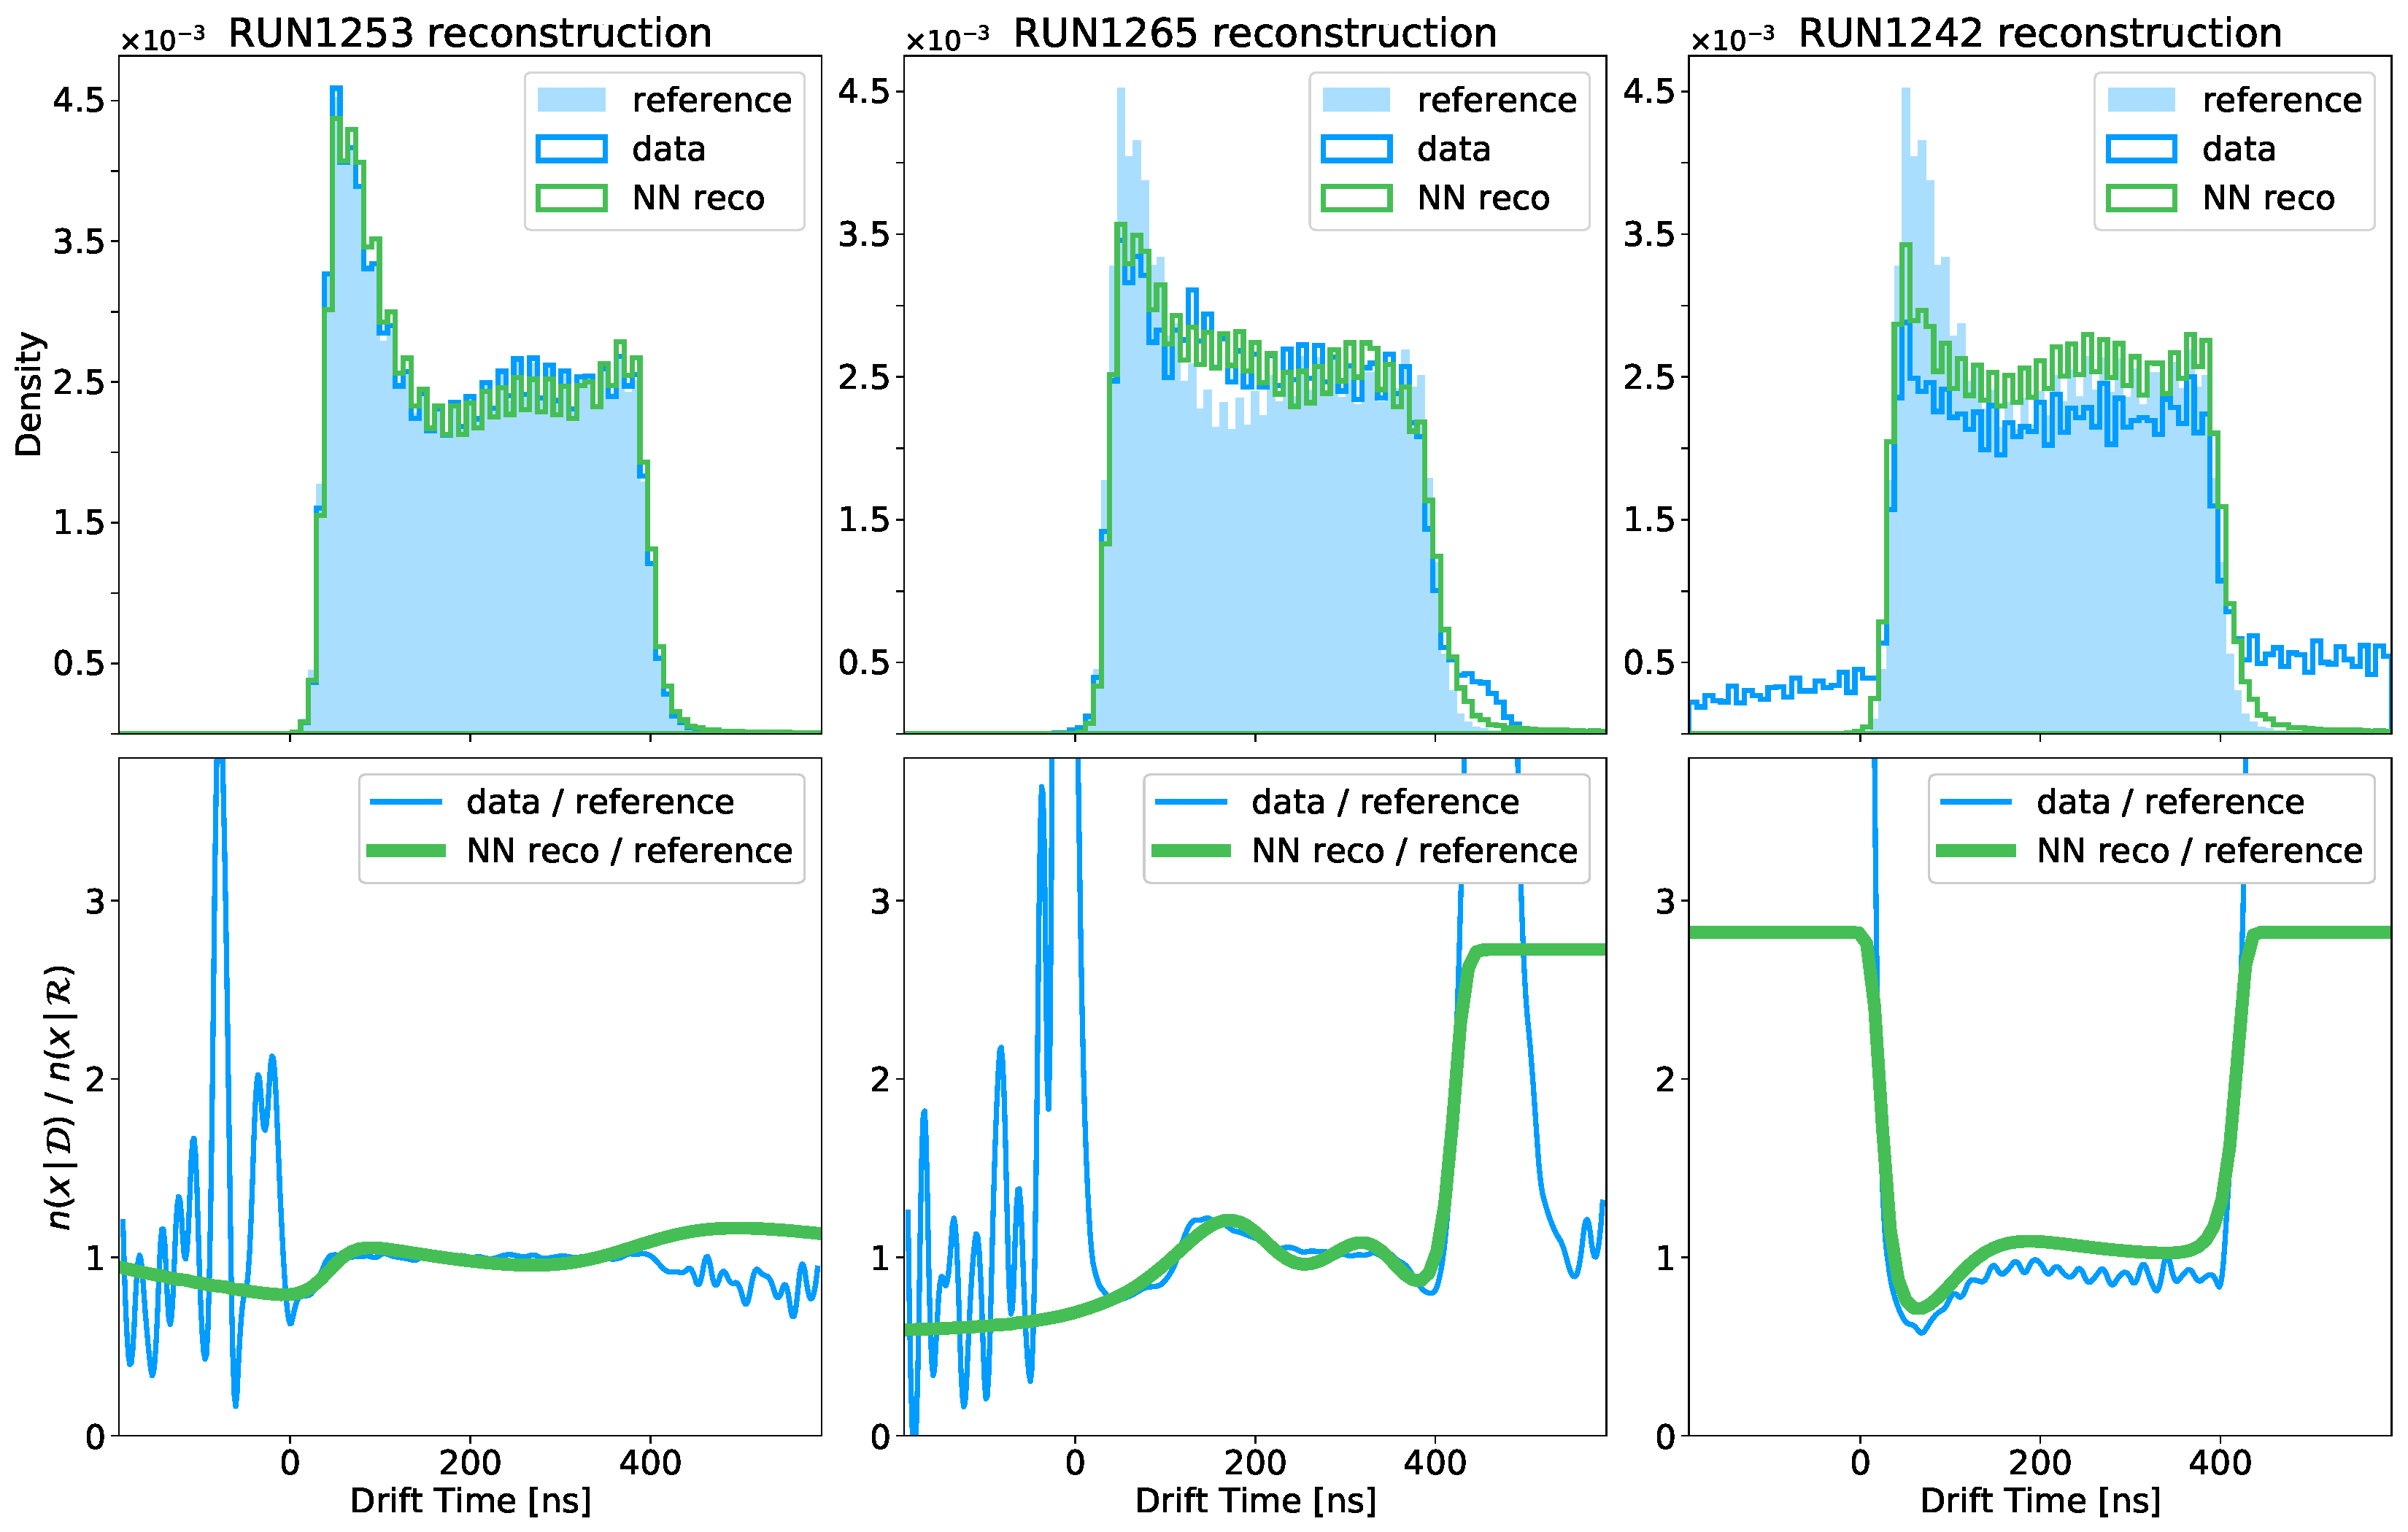
\includegraphics[width=1.0\textwidth]{../FALKON/plots/nn_reco.pdf}
    \caption{Neural network's data reconstruction for each of the three tested runs}
    \label{fig:reco}
\end{figure}

As we can see in \autoref{fig:reco}, the neural network can learn the ratio between $\D$ and $\R$ and grasp the overall
trend of it, but cannot reconstruct the strong discrepancies between the two accurately. Precisely, in the RUN1253
reconstruction, the algorithm does not detect relevant anomalies in $\D_{1253}$ (as we have already understood by
studying the observed test statistic $t_{\text{obs}}$) and thus the $n(x\,|\,\widehat{\mathbf{w}}) \, / \,
n(x\,|\,\mathbfcal{R})$ stays close to one. It is consistent with the empirical ratio inside the time box's range.
However, outside that range where the reference sample is almost not populated, the reconstruction is quite lacking, as
it cannot detect the fast oscillations of the ratio. The same behavior is reproduced in the RUN1265 reconstruction:
inside the $0\,-\,400\,\si{\nano\second}$ range, the reconstructed ratio fits the empirical one accurately. Here, the
network also detects the right-hand tail anomaly but does not have enough expressive power to reach the ratio's peak.
Similarly, the RUN1242 reconstruction does not fit the noise excess accurately outside the time box. This analysis of
the network's reconstruction shows us that the current implementation of the algorithm is not sufficient to understand
the data we are dealing with entirely. Of course, the algorithm stems from the search for new physics, where the
hoped-for signals have a low significance above the reference background. Thus, while sensitive to small departures from
$\R$, the algorithm fails to accurately understand substantial discrepancies if the NN's architecture is not complex
enough. However, our implementation can fit the overall trend of the ratio of the empirical distribution and
demonstrates that we are working in the right direction.














% \section{Future developments}

% We dedicate this last section of the chapter to quickly run through again our data quality monitoring concept and goal,
% introduced in \autoref{sec:DQM}, and assess what this thesis work had achieved and what is still missing out.

% \subsection{Automated monitoring}

% The first target of this work was to minimize the human efforts in data quality monitoring tasks. At this stage, a
% significant amount of human-performed work is necessary. However, this thesis laid the foundations for significant
% improvements. 

% Instead of having the scientist analyze the observed test statistic $t_{\text{obs}}$ at the end of the monitoring
% process and evaluate the quality of data, we would have the algorithm do it automatically. Namely, the idea could be to
% set two threshold values: the first one dividing the \textit{acceptable} $t_{\text{obs}}$ from the \textit{discrepant}
% $t_{\text{obs}}$ while the second one dividing the latter and the \textit{critical} $t_{\text{obs}}$. In other words,
% the two thresholds would define three regions in the space of the test statistic. Depending on which region the
% $t_{\text{obs}}$ belongs to, the algorithm would act in different ways: from just raising a warning to taking concrete
% actions towards the experimental setup. 

% However, to make this automated monitoring reliable, we must set meaningful and quantitative threshold values. The
% initial idea was to put those thresholds to the observed \textit{p}-value. As reported in \autoref{sec:disc_ass},
% though, we cannot make this idea concrete as for now. The alternative could be to put thresholds on the distance of
% $t_{\text{obs}}$ from the median $\tilde{t}$, though it does not seem satisfactory.

% Of even more importance, we would like to have threshold values that are as more universal as possible. Namely, we aim
% at having thresholds that do not depend (as far as possible) on the network's architecture and hyperparameters. It is a
% solid reason to consider median thresholds unsatisfactory, as they directly depend on the network's degrees of freedom.
% Moreover, through the numerous tests that we ran throughout this work, we noticed that the observed $t_{\text{obs}}$
% value is somehow unstable. In other words, if we feed to the network $N$ data sub-samples (instead of just one), we
% would find a distribution of $t_{\text{obs}}$ (the procedure is analogous to the tuning of the network). Its median
% could be used as an estimate of the overall observed test statistic and compared to the $p(t\,|\,\mathbfcal{R})$
% distribution. However, if the algorithm detects a discrepancy in the data samples, the $t_{\text{obs}}$ distribution
% will not follow a $\chi^2_{\nu}$ distribution. Instead, we found that the $t_{\text{obs}}$ distribute themselves
% following an approximate uniform distribution with considerable variance. Thus, even using data from the same run, the
% results are very variable and make it difficult to choose appropriate threshold values.

% A possible solution could be to have a more flexible neural network, and we thought of two possible implementations. The
% first one involves the employment of multiple reference samples. Namely, suppose the algorithm knows better what we
% label as \textit{good} run (by seeing more of them). In that case, it could have an improved evaluation of the test
% statistic and thus a more stable and reliable output. Possibly, this improvement could also lead to a reduction of the
% observed $t_{\text{obs}}$ values, making it possible to exploit the \textit{p}-value discrepancy assessment. However, a
% more straightforward solution could be to increase the network's complexity. This way, the algorithm would have an
% enhanced expressive power and could increase output reliability. 


% \subsection{Online monitoring}

% Even though increasing the network's complexity seem to solve most of the urging problems we have exposed, there is a
% substantial drawback that cannot be overlooked. 

% At the beginning of this chapter, we have stated that our goal is to build an \textit{online} data quality monitoring algorithm.
% By \textit{online} we mean "while the detector is collecting data". The functioning procedure of the algorithm we have
% in mind is thus the following: 

% \begin{itemize}
%     \item 
% \end{itemize}